\documentclass{article}

\usepackage{graphicx}
\usepackage{subcaption}
\usepackage{fancyhdr}
\usepackage[sorting=none]{biblatex}
\usepackage[margin=1in]{geometry}
\usepackage{listings}
\usepackage[hidelinks]{hyperref}
%\usepackage{subfigure}
\usepackage{amsmath}
\usepackage{float}
\usepackage{lmodern} % فونت بهتر برای لاتین
\usepackage{xcolor}
\usepackage{minted}
\usepackage{fvextra}

\setminted{
	linenos,
	breaklines=true,
	breakanywhere=true,
	encoding=utf8,
	autogobble=true,
	fontsize=\small,
	frame=single,
	tabsize=4,
	obeytabs=true,
	mathescape=false,
	texcomments=false
}
\usepackage{amssymb}
\usepackage{longtable} % برای جداول طولانی
\usepackage{enumitem} % برای کنترل لیست‌ها
\usepackage{booktabs} % برای جداول حرفه‌ای
\hypersetup{
	colorlinks=true,
	linkcolor=teal,
	filecolor=magenta,      
	urlcolor=teal,
	citecolor=teal
}
\usepackage{xepersian}




\setlength\headheight{28pt} 
\addbibresource{bibliography.bib}
\settextfont[Path={./font/}, Scale=1.3]{IRLotus}
\setlatintextfont[Scale=1]{Times New Roman}
\renewcommand{\baselinestretch}{1.5}
\pagestyle{fancy}
\fancyhf{}
\lhead{تمرین سری دوم رباتیک و بینایی ماشین}
\chead{
\includegraphics[width=1cm]{img/Logo.png}}
\rhead{\thepage}

\rfoot{محمدامین محمدیون شبستری}
\cfoot{هستی محمدی}
\lfoot{محمدسبحان سخایی}
\renewcommand{\headrulewidth}{1pt}
\renewcommand{\footrulewidth}{1pt}
\AtBeginDocument{
	\def\chapterautorefname{فصل}%
	\def\sectionautorefname{پاسخ سوال}%
	\def\subsectionautorefname{بخش}%
	\def\subsubsectionautorefname{بخش}%
	\def\equationautorefname{رابطهٔ}%
    \def\lstlistingautorefname{برنامۀ}%
}
\renewcommand{\lstlistingname}{Code}

\definecolor{codegreen}{rgb}{0,0.6,0}
\definecolor{codegray}{rgb}{0.5,0.5,0.5}
\definecolor{codepurple}{rgb}{0.58,0,0.82}
\definecolor{backcolour}{rgb}{0.95,0.95,0.92}

\lstdefinestyle{mystyle}{
	backgroundcolor=\color{backcolour},   
	commentstyle=\color{codegreen},
	keywordstyle=\color{magenta},
	numberstyle=\tiny\color{codegray},
	stringstyle=\color{codepurple},
	basicstyle=\ttfamily\footnotesize,
	breakatwhitespace=false,         
	breaklines=true,                 
	captionpos=b,                    
	keepspaces=true,                 
	numbers=left,                    
	numbersep=5pt,                  
	showspaces=false,                
	showstringspaces=false,
	showtabs=false,                  
	tabsize=2
}



\lstset{style=mystyle}

\begin{document}
\begin{titlepage}
\begin{center}
\defpersianfont\nast[Path={./font/}, Scale=1.8]{IranNastaliq}
\centerline{{
\includegraphics[width=4cm]{img/Logo.png}}}
\centerline{\textcolor[rgb]{0,0,0.5}{\nast \bfseries دانشکدۀ مهندسی برق}}

\vspace{0.5cm}

\huge
\textbf{درس رباتیک و بینایی ماشین}\\[0.4cm]
\textbf{استاد: دکتر حمیدرضا تقی راد}\\
\textbf{استاد: دکتر محمدجواد احمدی}\\
\textbf{تمرین سری دوم }\\
\textbf{گروه آزادی }\\
\vspace{0.4cm}

\begin{table}[ht]
\centering
\renewcommand{\arraystretch}{1.35}
\Large
\begin{tabular}{|c|c|}
\hline
نام و نام خانوادگی & محمدامین محمدیون شبستری\\
\hline
شمارهٔ دانشجویی & 40122503\\
\hline
نام و نام خانوادگی & محمدسبحان سخایی\\
\hline
شمارهٔ دانشجویی & 40119253\\
\hline
نام و نام خانوادگی & هستی محمدی\\
\hline
شمارهٔ دانشجویی & 40221243\\
\hline

تاریخ & فروردین 1405\\
\hline
%%\multicolumn{2}{|c|}{%
%%\begin{minipage}{0.9\linewidth}
%%\centering
%%\large
%%\textbf{لینک‌های مربوط به کد :}\\[0.3em]
%%\href{https://drive.google.com/file/d/1dC_vEO91lA3BBd1XWn54jxsrS-rq5QCG/view?usp=sharing}
%%{\textcolor{blue}{کد}}
%%\quad | \quad
%%\href{https://github.com/mobinamqdm/fundamentals-of-intelligent-systems-}
%%{\textcolor{blue}{لینک گیت‌هاب}}




%%\end{minipage}}\\
\hline
\end{tabular}
\end{table}

\vfill

\end{center}
\end{titlepage}



\tableofcontents \clearpage
\listoffigures \clearpage
\listoftables \clearpage
\lstlistoflistings \clearpage
\newpage

\section{سینماتیک مستقیم ربات \lr{KUKA iiwa}}

\subsection{استخراج DH}

\subsubsection{معرفی و بررسی قراردادهای دناویت-هارتنبرگ (DH)}

برای استخراج سینماتیک مستقیم ربات‌ها، دو قرارداد اصلی برای تعیین دستگاه‌های مختصات و استخراج پارامترهای دناویت-هارتنبرگ وجود دارد: قرارداد استاندارد \lr{(Standard DH)} و قرارداد اصلاح‌شده \lr{(Modified DH)}. در ادامه هر دو روش به طور کامل بررسی و مقایسه می‌شوند.

\paragraph{قرارداد استاندارد دناویت-هارتنبرگ \lr{(Standard DH)}}\mbox{}\\
این قرارداد که در سال ۱۹۵۵ معرفی شد، روش کلاسیک در سینماتیک رباتیک است. در این روش، دستگاه مختصات $i$ در انتهای لینک $i$ (روی مفصل $i+1$) قرار می‌گیرد. در این حالت، محور $z_{i-1}$ نشان‌دهنده راستای حرکت مفصل $i$ است و محور $x_i$ در امتداد عمود مشترک بین $z_{i-1}$ و $z_i$ تعریف می‌شود. ترتیب اعمال تبدیلات به صورت چرخش حول $z_{i-1}$، انتقال در راستای $z_{i-1}$، انتقال در راستای $x_i$ و در نهایت چرخش حول $x_i$ است. 

در مقالات علمی چاپ شده در ژورنال‌های معتبر مانند  \lr{SCIENCE DIRECT}، پارامترهای استخراج شده برای بازوی رباتیک (مانند \lr{KUKA LBR iiwa}) بر اساس قرارداد استاندارد معمولاً به شکل جدول \ref{tab:standard_dh} ارائه می‌شوند.

\begin{table}[htbp]
	\centering
	\caption{پارامترهای Standard DH (بر اساس مقالات مرجع)}
	\label{tab:standard_dh}
	\begin{tabular}{|c|c|c|c|c|}
		\hline
		مفصل ($i$) & $\alpha_i$ (رادیان) & $a_i$ (متر) & $d_i$ (متر) & $\theta_i$ (رادیان) \\ \hline
		1 & $-\pi/2$ & 0 & $d_1$ & $\theta_1$ \\ \hline
		2 & $\pi/2$ & 0 & 0 & $\theta_2$ \\ \hline
		3 & $\pi/2$ & 0 & $d_3$ & $\theta_3$ \\ \hline
		4 & $-\pi/2$ & 0 & 0 & $\theta_4$ \\ \hline
		5 & $-\pi/2$ & 0 & $d_5$ & $\theta_5$ \\ \hline
		6 & $\pi/2$ & 0 & 0 & $\theta_6$ \\ \hline
		7 & 0 & 0 & $d_7$ & $\theta_7$ \\ \hline
	\end{tabular}
\end{table}

\paragraph{قرارداد اصلاح‌شده دناویت-هارتنبرگ \lr{(Modified DH)}}\mbox{}\\
این قرارداد توسط جان کریگ \lr{(John J. Craig)} معرفی شد تا مشکلات روش استاندارد در ربات‌های دارای ساختار درختی را حل کند. در این روش، دستگاه مختصات $i$ در ابتدای لینک $i$ (روی خود مفصل $i$) قرار می‌گیرد. بنابراین، محور $z_i$ مستقیماً نشان‌دهنده محور چرخش مفصل $i$ است و محور $x_i$ در امتداد عمود مشترک بین $z_i$ و $z_{i+1}$ قرار دارد. ترتیب تبدیلات در این روش با چرخش و انتقال حول راستای محور $x_{i-1}$ شروع شده و با چرخش و انتقال حول راستای محور $z_i$ پایان می‌یابد.

\paragraph{مقایسه و انتخاب قرارداد مبنا برای مسئله حاضر}\mbox{}\\
تفاوت اصلی این دو قرارداد در محل قرارگیری فریم‌ها است؛ روش استاندارد فریم را در انتهای لینک (Distal) و روش اصلاح‌شده آن را در ابتدای لینک (Proximal) قرار می‌دهد. این تفاوت باعث می‌شود که در روش اصلاح‌شده، محور $z$ یک فریم دقیقاً منطبق بر مفصل متناظر خود باشد. 
با بررسی دقیق مختصات تعیین شده در شکل داده شده در صورت سوال، مشاهده می‌شود که دستگاه‌های مختصات دقیقاً منطبق بر قواعد \textbf{قرارداد اصلاح‌شده \lr{(Modified DH)}} رسم شده‌اند. بنابراین، مبنای ما برای حل این سوال و استخراج پارامترها، جدول \lr{Standard DH} ارائه شده در مقالات نیست، بلکه پارامترها باید بر اساس قواعد \lr{Modified DH} استخراج شوند.

\subsubsection{استخراج نهایی جدول DH بر اساس تصویر مسئله}

\paragraph{جدول پارامترهای DH اصلاح‌شده (مبنای حل)}\mbox{}\\
با توجه به دستگاه‌های مختصات رسم شده روی ربات که از قرارداد \lr{Modified DH} پیروی می‌کنند، پارامترهای دناویت-هارتنبرگ به صورت جدول \ref{tab:modified_dh} استخراج می‌گردند.

\begin{table}[htbp]
	\centering
	\caption{پارامترهای \lr{Modified DH} (استخراج شده از شکل مسئله)}
	\label{tab:modified_dh}
	\begin{tabular}{|c|c|c|c|c|}
		\hline
		مفصل ($i$) & $\alpha_{i-1}$ (رادیان) & $a_{i-1}$ (متر) & $d_i$ (متر) & $\theta_i$ (رادیان) \\ \hline
		1 & 0 & 0 & $d_1$ & $\theta_1$ \\ \hline
		2 & $-\pi/2$ & 0 & 0 & $\theta_2$ \\ \hline
		3 & $\pi/2$ & 0 & $d_3$ & $\theta_3$ \\ \hline
		4 & $\pi/2$ & 0 & 0 & $\theta_4$ \\ \hline
		5 & $-\pi/2$ & 0 & $d_5$ & $\theta_5$ \\ \hline
		6 & $-\pi/2$ & 0 & 0 & $\theta_6$ \\ \hline
		7 & $\pi/2$ & 0 & $d_7$ & $\theta_7$ \\ \hline
	\end{tabular}
\end{table}

\subsection{پیاده‌سازی سینماتیک مستقیم \lr{(Forward Kinematics Implementation)}}
در این بخش، به منظور محاسبه موقعیت نهایی مجری نهایی (End-Effector) نسبت به پایه ربات، یک برنامه مستقل به زبان پایتون توسعه داده شده است. با توجه به وجود دو استاندارد رایج در استخراج پارامترهای دناویت-هارتنبرگ، کد برنامه‌نویسی در دو حالت قرارداد اصلاح‌شده \lr{(Modified DH)} و قرارداد استاندارد \lr{(Standard DH)} پیاده‌سازی گردید تا صحت محاسبات ارزیابی شود.

در زیر، کدهای پیاده‌سازی شده برای هر دو حالت آورده شده است:
\subsubsection{کد}
\begin{LTR}
	\inputminted{python}{code/RC-Hw2-Q1.py}
\end{LTR}

\subsubsection{بررسی الگوریتم‌ها و ماتریس‌های تبدیل}
همان‌طور که در کدهای بالا مشاهده می‌شود، دو تابع مجزا برای تولید ماتریس‌های تبدیل همگن \lr{(Homogeneous Transformation Matrices)} نوشته شده است. تفاوت اصلی این دو پیاده‌سازی، در ترتیب ضرب ماتریس‌های پایه و در نتیجه قرارداد (Convention) استفاده شده است.

\paragraph{حالت اول: پیاده‌سازی بر اساس قرارداد اصلاح‌شده \lr{(Modified DH)}}\mbox{}\\ 
این حالت که بر اساس استاندارد جان کریگ \lr{(John J. Craig)} است، مختصات فریم $i$ را به مفصل $i$ متصل می‌کند. در تابع \texttt{mdh\_transformation\_matrix}، ترتیب ضرب ماتریس‌های انتقال و دوران به شکل زیر است:
$$ T_{i}^{i-1} = Rot_x(\alpha_{i-1}) \cdot Trans_x(a_{i-1}) \cdot Rot_z(\theta_i) \cdot Trans_z(d_i) $$
با ضرب این چهار ماتریس، ماتریس تبدیل کلی در استاندارد MDH به دست می‌آید که در کد پیاده‌سازی شده است:
$$ T_{MDH} = \begin{bmatrix} 
	\cos\theta_i & -\sin\theta_i & 0 & a_{i-1} \\ 
	\sin\theta_i \cos\alpha_{i-1} & \cos\theta_i \cos\alpha_{i-1} & -\sin\alpha_{i-1} & -d_i \sin\alpha_{i-1} \\ 
	\sin\theta_i \sin\alpha_{i-1} & \cos\theta_i \sin\alpha_{i-1} & \cos\alpha_{i-1} & d_i \cos\alpha_{i-1} \\ 
	0 & 0 & 0 & 1 
\end{bmatrix} $$

\paragraph{حالت دوم: پیاده‌سازی بر اساس قرارداد استاندارد \lr{(Standard DH)}}\mbox{}\\
این حالت که به قرارداد پاول \lr{(Paul's Convention)} نیز معروف است، فریم مختصات را به انتهای لینک متصل می‌کند. در تابع \texttt{dh\_transform}، ترتیب عملیات ریاضی متفاوت بوده و به صورت زیر تعریف می‌شود:
$$ T_{i}^{i-1} = Rot_z(\theta_i) \cdot Trans_z(d_i) \cdot Trans_x(a_i) \cdot Rot_x(\alpha_{i-1}) $$
که منجر به تولید ماتریس تبدیل زیر می‌گردد (متفاوت از حالت قبل):
$$ T_{Standard} = \begin{bmatrix} 
	\cos\theta_i & -\sin\theta_i \cos\alpha_i & \sin\theta_i \sin\alpha_i & a_i \cos\theta_i \\ 
	\sin\theta_i & \cos\theta_i \cos\alpha_i & -\cos\theta_i \sin\alpha_i & a_i \sin\theta_i \\ 
	0 & \sin\alpha_i & \cos\alpha_i & d_i \\ 
	0 & 0 & 0 & 1 
\end{bmatrix} $$

\subsubsection{تحلیل نتایج به دست آمده}
پس از اجرای اسکریپت‌ها بر روی سناریوهای تستی مختلف (حالت تمامی چرخش ها= صفر، چرخش ۹۰ درجه مفصل ۲ و چرخش ۹۰ درجه مفصل ۴)، مشاهده می‌کنیم که خروجی‌های عددی و موقعیت نهایی $(X, Y, Z)$ در هر دو پیاده‌سازی کاملاً یکسان است. 

به عنوان مثال در حالت تمامی چرخش ها= صفر برای هر دو الگوریتم داریم:
$$ P_{end-effector} = \begin{bmatrix} 0.0 \\ 0.0 \\ 1.266 \end{bmatrix} $$
و برای سناریوی دوم (انحراف مفصل دوم):
$$ P_{end-effector} = \begin{bmatrix} 0.926 \\ 0.0 \\ 0.34 \end{bmatrix} $$

\subsubsection{نتیجه‌گیری}
این تطابق دقیق نتایج، نشان‌دهندۀ صحت پیاده‌سازی هر دو الگوریتم است. اگرچه استانداردهای \lr{Modified DH} و \lr{Standard DH} در نحوۀ جایگذاری دستگاه‌های مختصات میانی \lr{(Intermediate Frames)} روی مفاصل و همچنین در فرمولاسیون ماتریس‌های انتقال با یکدیگر تفاوت ساختاری دارند، اما از آنجا که هر دو ساختار فیزیکی و سینماتیکیِ یکتای ربات \lr{(KUKA LBR iiwa)} را توصیف می‌کنند، ضرب ماتریس‌های آن‌ها از پایه تا مجری نهایی، در نهایت به یک موقعیت فضایی واحد و یکسان برای End-Effector ختم می‌شود.

\section{شبیه سازی سناریوی صنعتی سیستم بازرسی خودکار}
\subsection{بخش A --- پیاده‌سازی سیستم بینایی ماشین \lr{(OpenCV)}}
دوربینی که در بالای میز کار ربات نصب شده، مستقیما و عمود به پایین نگاه نمی‌کند، بلکه زاویه‌دار است. به همین دلیل، تصویری که به دست ما می‌رسد دچار اعوجاج پرسپکتیو  \lr{(Projective / Keystone Distortion)} شده و کمی هم نویز ملایم گوسی \lr{(Gaussian Noise)} دارد. روی این میز کار، چهار نشانگر مربعی و مشکی‌رنگ در گوشه‌ها قرار داده شده‌اند که یک فضای کاری مربعی به ابعاد دقیق $0.6 \times 0.6$ متر را مشخص می‌کنند. در داخل این فضا، چند دیسک رنگی به عنوان قطعات هدف قرار گرفته‌اند.

\paragraph{قرارداد مختصات در این مسئله}\mbox{}\\
اگر از گوشه بالا و سمت چپ میز کار فیزیکی شروع کنیم و در جهت عقربه‌های ساعت بچرخیم، موقعیت این چهار نشان‌گر مشکی در دستگاه مختصات پایه ربات به صورت زیر تعریف می‌شود (همه واحدها بر حسب متر هستند): 

\begin{table}[htbp]
	\centering
	\caption{مختصات نشانگرها در دستگاه مختصات پایه ربات}
	\label{tab:coordinates}
	\begin{tabular}{|c|c|c|c|c|}
		\hline
\lr{TL} & بالا-چپ & $(+0.30, +0.30)$ \\ \hline
\lr{TR} & بالا-راست & $(+0.30, -0.30)$ \\ \hline
\lr{BR} & پایین-راست & $(-0.30, -0.30)$ \\ \hline
\lr{BL} & پایین-چپ & $(+0.30, +0.30)$ \\ \hline
	\end{tabular}
\end{table}


فرض کنید پایه ربات دقیقا در نقطه مرکزی و زیر میز کار محکم شده است. همچنین سطح میز کار، صفحه $z = 0 $ در مختصات چهانی در نظر گرفته شود.

\subsubsection{تسک \lr{A.1} --- شبیه‌سازی و تولید تصویر میز کار}

در محیط واقعی صنعتی ،تصویر مستقیما از دوربین گرفته می‌شود، اما در این تمرین تصویر دوربین با استفاده از کد داده شده شبیه‌سازی شده است. این کد به دست نخورده باقی‌مانده و تنها کتابخانه‌های لازم برای اجرای آن در سه خط ابتدایی اضافه شده‌اند.


\begin{latin}
\begin{LTR}
\begin{verbatim}
import cv2
import numpy as np
import matplotlib.pyplot as plt
\end{verbatim}
\end{LTR}
\end{latin}



تصویر تولید شده (شکل \ref{fig:out}) شامل موارد زیر است:
\begin{itemize}
\item چهار مربع مشکی در گوشه‌ها که برای کالیبره کردن استفاده می‌شوند.
\item پنج دیسک رنگی که مختصات واقعی و دقیق آن‌ها در متغیر \mintinline{python}{GROUND_TRUTH_DISCS} ذخیره شده است.
\item شبیه‌سازی زاویه دوربین، اثر تاریکی گوشه‌های لنز \lr{(Vignetting)} و کمی نویز طبیعی تصویر.
\end{itemize}

\begin{figure}[H]
    \centering
    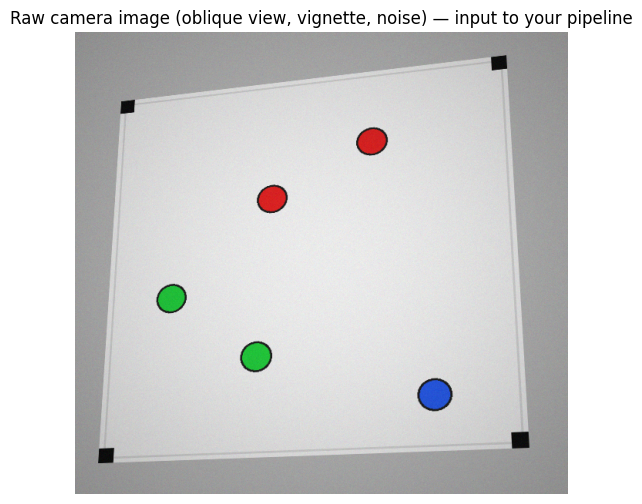
\includegraphics[width=0.8\textwidth, keepaspectratio]{output.png}
    \caption{تصویر شبیه‌سازی شده (تصویر دوربین)}
    \label{fig:out}
\end{figure}

\subsubsection*{خطاهای رایج در تصویربرداری}\mbox{}\\

در یک سامانهٔ بینایی ماشین کیفیت داده ورودی نقش تعیین‌کننده‌ای در عملکرد کل پایپ‌لاین پردازش تصویر دارد. تصویر ثبت‌شده توسط یک دوربین معمولی هرگز ایده‌آل نیست و معمولاً شامل انواع مختلفی از اعوجاج‌ها و خطاها است که در تصویر ورودی این مسئله شامل اعوجاج پرسپکتیو، نویز گاوسی و اثر تاریکی گوشه‌های لنز است.

وجود این خطاها می‌تواند مراحل بعدی پردازش تصویر مانند مشخص کردن گوشه‌ها، استخراج نشانگرها، تخمین ماتریس هموگرافی و تبدیل مختصات تصویر به مختصات واقعی را با خطا مواجه کند. در نتیجه اگر این خطاها در همان ابتدا مدل‌سازی و اصلاح نشوند، در مراحل بعدی تقویت شده و منجر به پدیده‌ \lr{GIGO} یا \lr{Garbage In, Garbage Out} می‌شوند که به معنای نتیجه نامطلوب در اثر ورودی نامناسب است. به همین دلیل در طراحی یایپ‌لاین، معمولاً مرحله‌ای برای پیش‌پردازش تصویر در نظر گرفته می‌شود که شامل اصلاح خطاها است و هدف آن تولید داده‌ای پایدار و قابل اعتماد برای مراحل بعدی است.

\paragraph{اعوجاج پرسپکتیو \lr{(Keystone Distortion)}:}\mbox{}\\
اگر در هنگام تصویربرداری از صحنه مورد نظر، دوربین کاملا عمود قرار نگرفته باشد، تصویر ثبت‌شده دچار اعوجاج پرسپکتیو می‌شود و خطوطی که در فضای واقعی موازی هستند ممکن است در تصویر همگرا به نظر برسند. بر فرض مثال در این مسئله، به علت مایل بودن دوربین نسبت به صفحه میز، مربع‌های کالیبراسیون که در واقعیت شکل کاملاً مربعی دارند، در تصویر به صورت ذوزنقه یا متوازی‌الاضلاع دیده می‌شوند. 

این خطا با تخمین ماتریس هموگرافی از روی نقاط متناظر، قابل اصلاح است و تصویر به نمایی معادل با دید عمود بر میز تبدیل می‌شود که این عمل اصلاح پرسپکتیو \lr{(Perspective Rectification)} نام دارد و یکی از اجزای کلیدی در تبدیل مختصات تصویر به مختصات دنیای واقعی است.

\paragraph{ نویز گاوسی \lr{(Guassian Noise)}:}\mbox{}\\
یکی دیگر از مشکلات رایج در تصاویر ثبت شده دوربین نویز سنسور است. سنسورهای تصویری به دلیل محدودیت‌های الکترونیکی و حرارتی دچار نوسانات تصادفی در اندازه‌گیری شدت نور می‌شوند. این نویز باعث می‌شود مقدار شدت روشنایی پیکسل‌ها به طور تصادفی تغییر کند. در نتیجه لبه‌ها و مرزهای اشیاء ممکن است کمی محو شده و آشکارسازی گوشه یا لبه دچار خطا شوند. به همین دلیل معمولاً پیش از استخراج داده‌ها و ویژگی‌های لازم از یک فیلتر برای کاهش اثر آن استفاده می‌شود. 

 نویز ناشی از سنسورهای تصویری دوربین به طور معمول با یک توزیع گاوسی مدل‌سازی شده و نویز گاوسی نامیده می‌شود. مدل ریاضی متداول برای نویز گاوسی به صورت زیر است

\[
I_{measured}(x,y) = I_{true}(x,y) + n(x,y)
\]

که در آن $I_{true}$ تصویر واقعی و $I_{measured}$ تصویر ثبت‌شده توسط دوربین است. عبارت $n(x,y)$ نیز به شکل زیر تعریف شده  

\[
n(x,y) \sim \mathcal{N}(0,\sigma^2)
\]

و نویز گاوسی با توزیع $\sigma$ را نشان می‌دهد که مقدار آن میزان شدت نویز را تعیین می‌کند.

یکی از رایج‌ترین روش‌ها استفاده از فیلتر گاوسی است که با میانگین‌گیری وزن‌دار در یک همسایگی محلی، نوسانات فرکانس بالا را کاهش می‌دهد.

\paragraph{اثر تاریکی گوشه‌های لنز \lr{(Vignetting)}:}\mbox{}\\
اثر تاریکی گوشه‌های لنز، یکی دیگر از خطاهای رایج در سیستم‌های تصویربرداری است که در آن روشنایی تصویر در نواحی پیرامونی کمتر از مرکز تصویر است. این پدیده معمولاً به دلیل طراحی اپتیکی لنز، محدودیت‌های مکانیکی یا افت شدت نور در مسیر اپتیکی ایجاد می‌شود.

این تغییر تدریجی در روشنایی می‌تواند الگوریتم‌هایی را که بر اساس آستانه‌گذاری یا مقایسهٔ شدت روشنایی کار می‌کنند دچار مشکل کند. برای مثال در این مسئله، یک یک نشانگر سیاه در مرکز تصویر ممکن است به راحتی از پس‌زمینه تمایز داده شود، اما همان نشانگر در گوشه تصویر به دلیل تاریک‌تر بودن پس‌زمینه ممکن است به درستی تشخیص داده نشود.

یک مدل ساده برای این پدیده تعریف یک تابع  وابسته به فاصله از مرکز تصویر است که در تصویر واقعی ضرب می‌شود. این تابع معمولا به صورت شعاعی تعریف شده و با افزایش فاصله از مرکز تصویر کاهش می‌یابد و در رابطه زیر با $V(x, y)$ نمایش داده شده است:
\[
I_{measured}(x,y) = V(x,y) \cdot I_{true}(x,y)
\]

\subsubsection{تسک \lr{A.2} --- شناسایی چهار نشانگر گوشه میز}
هدف این قسمت نوشتن برنامه‌ای است که بتواند چهار مربع مشکی (نشانگرهای کالیبراسیون) را پیدا کند. خروجی باید آرایه‌ای از مختصات این چهار نقطه باشد که حتما به ترتیب ساعت‌گرد و شروع از گوشه بالا--چپ تصویر \lr{(TL, TR, BR, BL} مرتب شده باشند. این ترتیب‌بندی برای هماهنگی با آرایه موقعیت جهانی در مراحل بعدی الزامی‌ است.

برای تعیین نواحی نشانگرهای مربعی مشکی به صورت پایدار و قابل اعتماد، انتخاب نحوه نمایش تصویر و تعریف درست آستانه‌ها الزامی است و در مراحل بعدی پایپ‌لاین نقش اساسی و تعیین‌کننده‌ای دارد.

بنابراین برای پاسخ به این سوال لازم است:
\begin{enumerate}
\item فضای رنگی مناسب انتخاب شود.
\item مقدار مناسب آستانه بر روی کانال درست از فضای تصویر اعمال شود تا نواحی مشکی نشانگرها از پس‌زمینه جداسازی شوند.
\item کانتورها از تصویر باینری استخراج شوند.
\item مرز‌ها و لبه‌ها آشکار و مشخص شوند.
\end{enumerate}

\paragraph{فضاهای رنگی \lr{(Color Spaces)} و تاثیر آن‌ها بر پردازش تصویر}\mbox{}\\
فضاهای رنگی، نحوه سازماندهی اطلاعات رنگی یک تصویر را مشخص می‌کنند. با انتخاب فضای مناسب برای تصویر قبل از شروع فرآیند، می‌توان سرعت پردازش و پایداری عملکرد در شرایط نوری متغیر را افزایش داد.

چند فضای رنگی رایج عبارت‌اند از:
\begin{description}
\item{\lr{RGB}:}
تصویر خامی که از دوربین دریافت می‌شود، معمولاً در فضای رنگی \lr{RGB} نمایش داده می‌شود که در آن، هر پیکسل با سه مؤلفه رنگی توصیف می‌شود؛ یعنی برای هر پیکسل، سه مقدارمعین بین $0$ تا $255$ نشان‌دهنده شدت رنگ‌های قرمز، سبز و آبی هستند. 
 
از نظر هندسی اگر در مختصات کارتزین \lr{(Cartesian Coordinates)} سه محور $x$--$y$--$z$ را به ترتیب شدت رنگ‌های قرمز، سبز و آبی فرض کنیم، فضای \lr{RGB} در داخل یک مکعب با ضلع $256$ قرار می‌گیرد و دو راس از این مکعب به مختصات‌های $(0, 0, 0)$ و $(255, 255, 255)$ به ترتیب نشان‌دهنده مشکی و سفید هستند.

بنابراین در این فضا، شدت روشنایی و اطلاعات رنگی درهم‌‌آمیخته شده‌اند و در نتیجه تصویر رنگی در فضای \lr{RGB} نسبت به تغییرات در روشنایی و تاریکی بسیار حساس هستند. این مسئله باعث می‌شود که این نمایش برای برخی از اهداف در بینایی ماشین انتخاب مناسبی نباشد.

\item{\lr{HSV(Hue, Saturation, Value)}:}
در فضای \lr{HSV} هر پیکسل با سه مؤلفه رنگ \lr{(Hue)}، شدت رنگ \lr{(Saturation)} و شدت نور \lr{(Value)} مشخص می‌شود. جداسازی رنگ از شدت روشنایی باعث می‌شود که این فضا نسبت به \lr{RGB} بیشتر مورد استفاده قرار بگیرد.

از نظر هندسی، این فضا همان مدل \lr{RGB} را در مختصات استوانه‌ای نمایش می‌دهد؛ به طوری که سه مؤلفه $(r, \theta, z)$ معادل $(S, H, V)$ می‌باشند.
\item{\lr{Grayscale}:}
در فضای \lr{Grayscale}، تمام اطلاعات رنگی حذف شده و تنها شدت روشنایی به صورت یک تابع اسکالر نگه داشته می‌شود. در نتیجه در زمان‌هایی که به دنبال مشخص کردن نواحی خیلی تیره یا خیلی روشن هستیم، استفاده از این فضا می‌تواند سرعت پردازش را به حداکثر برساند.

\item{\lr{LAB (CIELAB)}:}
فضای \lr{LAB} کل بازه رنگ‌هایی که انسان توانایی دیدنشان را دارد را در بر گرفته و به علت جداسازی شدت روشنایی از اطلاعات رنگی، پایدارترین عملکرد را در محیط طبیعی با شدت روشنایی‌های متغیر دارد. مؤلفه‌ $L$ شدت روشنایی، $A$ شدت رنگ‌های متضاد سبز (سمت منفی) و قرمز (سمت مثبت) و $B$ شدت رنگ‌های متضاد آبی (در سمت منفی) و زرد (در سمت مثبت) را نشان می‌دهند.

\end{description}

\paragraph{تعریف آستانه \lr{(Threshold)}}\mbox{}\\
با تعریف آستانه روی کانال‌های فضای رنگی، می‌توان تصویر را به یک تصویر باینری تبدیل کرد، به طوری که پیکسل‌هایی که از یک شرط مشخص پیروی می‌کنند در یک گروه و بقیه در گروهی دیگر قرار داده می‌شوند. آستانه‌گذاری به دو روش سراسری و تطبیقی انجام می‌شود.

در آستانه‌گذاری سراسری یک مقدار آستانه ثابت برای کل تصویر انتخاب می‌شود و اگر فرض شود که آستانه $T$ روی یک کانال از فضای رنگی تعریف شده و $I(x, y)$ مقدار آن مؤلفه‌ در یک پیکسل دلخواه را نشان می‌دهد، می‌توان نوشت: 

\[
B(x,y) =
\begin{cases}
1 & I(x,y) < T \\
0 & I(x,y) \geq T
\end{cases}
\]
این روش با وجود  ساده یودن، نسبت به تغییرات روشنایی حساس است. 

در آستانه‌گذاری تطبیقی، برای هر ناحیه از تصویر آستانه بر اساس همسایگی محلی تعیین شده و تابعی از مکان تصویر است. به صورت ریاضی می‌توان نوشت:

\[
B(x,y) =
\begin{cases}
1 & I(x,y) < T(x,y) \\
0 & I(x,y) \geq T(x,y)
\end{cases}
\]

که در آن $T(x,y)$ معمولاً بر اساس میانگین وزن‌دار مؤلفه مشخص‌شده در همسایگی پیکسل محاسبه می‌شود.

این روش در حضور \lr{vignetting}، سایه‌ها و روشنایی‌های ناهمگن پایدارتر است.


\paragraph{کانتور \lr{(Contour)} و لبه \lr{(Edge)}}\mbox{}\\
پس از باینری کردن تصویر، نواحی متصل مربوط به اشیاء قابل استخراج هستند. 

مجموعه‌ نقاطی که در آن‌ها تغییر شدت روشنایی زیاد است را لبه می‌نامند. لبه یک مفهوم گرادیانی است که معمولا روی اندازهٔ گرادیان شدت روشنایی تعریف می‌شود. اگر $I(x,y)$ شدت روشنایی باشد، گرادیان به صورت زیر تعریف می‌شود:

\[
\nabla I(x,y) =
\begin{bmatrix}
\frac{\partial I}{\partial x} \\
\frac{\partial I}{\partial y}
\end{bmatrix}
\]
اندازهٔ گرادیان نیز با

\[
\|\nabla I(x,y)\| = \sqrt{\left(\frac{\partial I}{\partial x}\right)^2 + \left(\frac{\partial I}{\partial y}\right)^2}
\]

برابر است و نشان می‌دهد که شدت روشنایی در تصویر با چه سرعتی تغییر می‌کند. نقاطی که این مقدار در آن‌ها بزرگ است، کاندیدهای لبه هستند.

در مقابل، کانتور معمولاً مرز هندسی بسته پیرامون ناحیه یک شیء است. در یک تصویر باینری شده کانتور مرز میان نواحی با مقدار ۱ و ۰ را نشان می‌دهد و برای توصیف شکل جسم، محاسبهٔ مساحت، محیط و مرکز هندسی مناسب‌تر است.


\paragraph{کد پیاده‌سازی شده و توضیحات آن}\mbox{}\\
\addcontentsline{lol}{lstlisting}{کد تسک \lr{A.2}}
\begin{latin}
\begin{LTR}
\begin{minted}{python}
import cv2
import numpy as np

def detect_corner_markers(image):
    """
    Find the 4 black square calibration markers.
    Returns: corners array sorted [TL, TR, BR, BL]
    """

    # brg --> hsv
    hsv = cv2.cvtColor(image, cv2.COLOR_BGR2HSV)

    # threshold 
    _, binary = cv2.threshold(
        hsv[:, :, 2],
        50,
        255,
        cv2.THRESH_BINARY_INV
    )

    # external contours
    contours, _ = cv2.findContours(
        binary,
        cv2.RETR_EXTERNAL,
        cv2.CHAIN_APPROX_SIMPLE
    )

    # filter by size & squareness
    square_candidates = []

    for cnt in contours:
        area = cv2.contourArea(cnt)

        if area < 100:
            continue

        x, y, w, h = cv2.boundingRect(cnt)

        box_area = w * h
        squareness = area / box_area if box_area > 0 else 0

        if squareness > 0.3:
            square_candidates.append(cnt)

    # largest 4
    square_candidates.sort(key=cv2.contourArea, reverse=True)
    top4 = square_candidates[:4]

    if len(top4) < 4:
        raise ValueError("Could not detect 4 corner markers")

    # centroids
    centers = []

    for cnt in top4:
        M = cv2.moments(cnt)

        if M['m00'] == 0:
            continue

        cx = int(M['m10'] / M['m00'])
        cy = int(M['m01'] / M['m00'])

        centers.append((cx, cy))

    # sort
    centers = sort_clockwise(centers)

    return np.float32(centers)


def sort_clockwise(pts):
  
    pts = sorted(pts, key=lambda p: p[1])

    top = sorted(pts[:2], key=lambda p: p[0])
    bottom = sorted(pts[2:], key=lambda p: p[0], reverse=True)

    return [top[0], top[1], bottom[0], bottom[1]]


# load image
image_path = r"C:\Users\Asus\Desktop\hasti\output.png"   # change to your image path
image = cv2.imread(image_path)

if image is None:
    raise FileNotFoundError(f"Image not found: {image_path}")

# detect markers
corners = detect_corner_markers(image)

print("Detected corners:")
print(corners)

# draw detected points
output = image.copy()

labels = ["TL", "TR", "BR", "BL"]

for i, (x, y) in enumerate(corners.astype(int)):
    cv2.circle(output, (x, y), 10, (0, 0, 255), -1)

    cv2.putText(
        output,
        labels[i],
        (x + 10, y - 10),
        cv2.FONT_HERSHEY_SIMPLEX,
        0.7,
        (0, 255, 0),
        2
    )

# save & show
cv2.imwrite("detected_markers.jpg", output)
cv2.imshow("Detected Markers", output)
cv2.waitKey(0)
cv2.destroyAllWindows()


\end{minted}
\end{LTR}
\end{latin}

در مسئله فعلی هدف تشخیص نشانگرهای سیاه است، بنابراین فضاهای رنگی که در آن روشنایی از رنگ متمایز شده (مانند \lr{Grayscale} یا \lr{HSV}) انتخاب مناسب‌تری هستند؛ چرا که وجه تمایز این نشانگرها نسبت به زمینه تیره بودن آن‌ها است نه رنگ. علاوه بر این می‌دانیم روشنایی تصویر یکنواخت نیست و اثر تاریکی گوشه‌های لنز وجود دارد.

بنابراین دو راه پیش رو، تبدیل تصویر به \lr{Grayscale} و استفاده از آستانه‌گذاری تطبیقی یا تبدیل تصویر به \lr{HSV} و تعریف یک آستانه برای کانال روشنایی \lr{(Value)} هستند. روش اول حجم مسئله و داده‌ها را کاهش می‌دهد، با این حال در روش دوم، اعمال آستانه سراسری کافی است و به علاوه در تسک \lr{A.4} برای پیدا کردن دیسک‌های رنگی، دیگر نیازی به تبدیل دوباره تصویر به \lr{HSV} نیست. در نتیجه عکس را در ابتدا به \lr{HSV} تبدیل می‌کنیم. در این فضا \lr{Value} رنگ مشکی صفر است، پس \lr{Value} پیکسل‌ها باید از حد آستانه انتخاب شده برای باینری کردن \lr{(Binarization)} تصویر کوچکتر باشند.

در تعیین مقدار آستانه نه باید آنقدر سخت‌گیرانه عمل کنیم که نشانگرها در تصویر باینری غیرقابل تشخیص شوند و نه باید آنقدر محدوده را باز بگذاریم که تاریکی‌ها و سایه‌های تصویر اجاره تشخیص درست نشانگرها را از ما بگیرند. بدین منظور، پس از کمی آزمون و خطا مقدار آستانه برای رنگ مشکی در کد $50$ در نظر گرفته شده است.

در مرحله بعدی به دنبال استخراج کانتورها می‌رویم که در اینجا کاربردی‌تر از اتکا به لبه‌هاست، زیرا می‌توانیم مرز بسته نشانگرهای مربعی تیره را پس از باینری کردن تصویر مستقیما به صورت کانتور استخراج کنیم.

حال برای جدا کردن این 4 نشانگر از دیگر نویزها، کانتورها را بر اساس مساحت و مربع بودن فیلتر می‌کنیم. برای این کار ابتدا مساحت هر کانتور را به دست آورده و اگر این مساحت کوچکتر از $100$ باشد، کانتور متناظر از لیست کاندیدها حذف می‌شود. سپس مساحت کانتورهای باقی‌مانده را بر مساحت کوچکترین مستطیلی که محیط بر آن است \lr{(Bounding Rectangle)} تقسیم می‌کنیم و اگر حاصل تقسیم از $0.3$ بزرگتر باشد، به لیست کاندیدها اضافه می‌شود. در نهایت چهار کاندیدی که بیشترین مساحت را دارند انتخاب شده، مرکز آنها محاسبه می‌شود و به ترتیب ساعت‌گرد با شروع از گوشه بالا-چپ مرتب می‌شوند.

\paragraph{خروجی کد}\mbox{}\\
تصویر خروجی این کد در شکل \ref{fig:1} آمده است.
\begin{figure}[H]
    \centering
    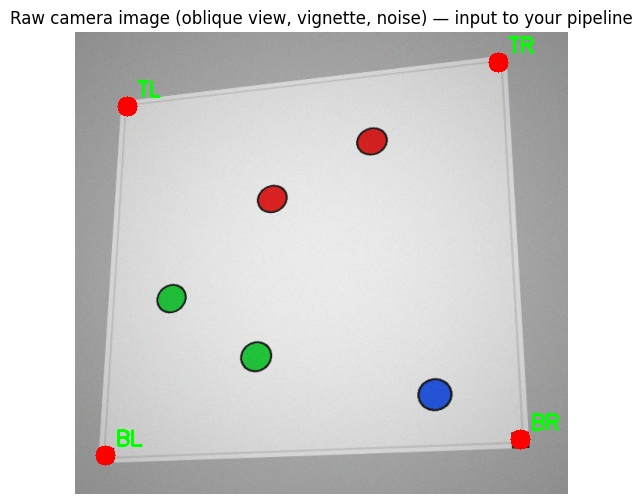
\includegraphics[width=0.8\textwidth, keepaspectratio]{dm.jpg}
    \caption{مشخص کردن نشانگرها روی تصویر به ترتیب ساعتگرد}
    \label{fig:1}
\end{figure}

خروجی دیگر کد این بخش، مختصات پیکسلی چهار نشانگر است که به صورت زیر است:
\begin{latin}
	\begin{verbatim}
Detected corners:
[[127. 106.]
 [498.  62.]
 [520. 439.]
 [105. 455.]]
	\end{verbatim}
\end{latin}

\subsubsection{تسک \lr{A.3} --- اصلاح پرسپکتیو تصویر (تبدیل به نمای عمودی)}
در این تسک، با داشتن مختصات پیکسلی چهار گوشه و مختصات واقعی آن‌ها روی میز کار، ماتریس هوموگرافی \lr{(Homography Matrix)} را به دست آورده و با استفاده از آن تصویر مایل دوربین را به تصویر جدیدی به اندازه $600 \times 600 $ پیکسل از نمای کاملا بالا به پایین \lr{(Top-Down)} تبدیل می‌کنیم.

برای تصویر جدید شرط‌های زیر وجود دارد:
\begin{enumerate}
\item نقطه مرکزی میز کار باید دقیقا در وسط تصویر یعنی پیکسل $(300, 300)$ قرار بگیرد.
\item هر 1 متر در دنیای واقعی باید معادل با 1000 پیکسل در تصویر باشد (با این مقیاس، میز 60 در 60 سانتی‌متری دقیقا کل ادر 600 در 600 پیکسلی را پر می‌کند).
\item ضریب تبدیل پیکسل به متر باید در کد تعریف شود و برای اطمینان از صحت کار، یک شبکه شطرنجی \lr{(Grid)} با فاصله‌های 6 سانتی‌متری روی تصویر اصلاح شده رسم شود.
\end{enumerate}

\paragraph{ماتریس هوموگرافی}\mbox{}\\
از آن‌جا که میز یک صفحه در فضای سه‌بعدی است و تمام نشانگرها روی صفحه $z = 0 $ قرار دارند، می‌توان رابطه‌ای مستقیم بین نقاط روی صفحه میز و پیکسل‌های تصویر دوربین برقرار کرد. همانطور که پیشتر نیز گفته شد، چون دوربین نسبت به میز زاویه دراد، مربع‌های روی میز در تصویر به شکل ذوزنقه دیده شده و موازی‌ها در تصویر همگرا می‌شوند. 

ماتریس هوموگرافی ابزاری است که این اعوجاج پرسپکتیو را مدل می‌کند؛ یعنی با داشتن چهار نقطه گوشه (در این مسئله چهار نشانگر \lr{TL, TR, BR, BL}) می‌توان تبدیل را تخمین زد و سپس تصویر را طوری \lr{Warp} کرد که صفحه میز مانند حالتی که دوربین دقیقاً عمود بر آن است مشاهده شود. این ماتریس یک تبدیل \lr{Projective} بین دو صفحه است که در مختصات همگن نمایش داده می‌شود. 

اگر یک نقطه در تصویر ورودی $\mathbf{p} = \begin{bmatrix} x \\ y \\ 1 \end{bmatrix}$ و نقطه متناظر آن در تصویر خروجی اصلاح شده $\mathbf{p}' = \begin{bmatrix} x' \\ y' \\ 1 \end{bmatrix}$ باشد، داریم:

\[
\mathbf{p}' \sim \mathbf{H}\mathbf{p}
\]

که $\mathbf{H}$ یک ماتریس $3 \times 3$ است به شکل زیر است:

\[
\mathbf{H}=
\begin{bmatrix}
h_{11} & h_{12} & h_{13} \\
h_{21} & h_{22} & h_{23} \\
h_{31} & h_{32} & h_{33}
\end{bmatrix}
\]

 با بازنویسی رابطه، مختصات اقلیدسی خروجی از تقسیم بر مولفه سوم به دست می‌آید:

\[
\begin{bmatrix}
\tilde{x}' \\
\tilde{y}' \\
\tilde{w}'
\end{bmatrix}
=
\mathbf{H}
\begin{bmatrix}
x \\
y \\
1
\end{bmatrix},
\quad
x'=\frac{\tilde{x}'}{\tilde{w}'},
\quad
y'=\frac{\tilde{y}'}{\tilde{w}'}
\]

از آن‌جا که $\mathbf{H}$ دارای 9 مولفه است ولی فقط تا یک مقیاس معنا دارد، 8 درجه آزادی دارد؛ لذا حداقل 4 نقطه غیرهم‌خط متناظر برای حل آن لازم است. در این مسئله چهار نشانگر کالیبراسیون روی گوشه‌های میز چنین نقاطی را فراهم می‌کنند. 

به صورت کاربردی، اگر چهار گوشه میز در تصویر دوربین مشخص شوند و چهار نقطه مقصد در صفحه خروجی تعیین گردد، می‌توان تصویری ساخت که در آن صفحه میز مستطیلی و با مقیاس مطلوب نمایش داده شود.

\paragraph{کد پیاده‌سازی شده و توضیحات آن}\mbox{}\\
برای پیاده‌سازی این قسمت کافی است:
\begin{enumerate}
\item ابتدا یک تصویر خالی به اندازه $600 \times 600 $ تولید کنیم.
\item با استفاده از مختصات فعلی و مقصد نشانگرها و دستور \mintinline{python}{cv2.findHomography}  ماتریس هوموگرافی را محاسبه می‌کنیم.
\item در نهایت تصویر با استفاده از \mintinline{python}{cv2.warpPerspective} به نمای بالا به پایین تبدیل می‌شود.
\end{enumerate}

برای به دست آوردن نمای کاملا بالا به پایین و مرکز تصویر قبل و بعد از تصحیح پرسپکتیو، کد زیر نوشته شده است:
\addcontentsline{lol}{lstlisting}{کد تسک \lr{A.3}}

\begin{latin}
\begin{LTR}
\begin{minted}{python}

original_display = image.copy()

# center
p1 = corners[0]
p2 = corners[2]

p3 = corners[1]
p4 = corners[3]

x1, y1 = p1.astype(np.float64)
x2, y2 = p2.astype(np.float64)

x3, y3 = p3.astype(np.float64)
x4, y4 = p4.astype(np.float64)

# p1 - p2
A1 = y2 - y1
B1 = x1 - x2
C1 = A1 * x1 + B1 * y1

# p3 - p4
A2 = y4 - y3
B2 = x3 - x4
C2 = A2 * x3 + B2 * y3

det = A1 * B2 - A2 * B1

if abs(det) < 1e-10:
    raise ValueError("Diagonal lines are parallel or ill-conditioned.")

center_x = (B2 * C1 - B1 * C2) / det
center_y = (A1 * C2 - A2 * C1) / det

draw_center_x = int(round(center_x))
draw_center_y = int(round(center_y))

old_center = np.array([[[center_x, center_y]]], dtype=np.float32)

cv2.circle(
    original_display,
    (draw_center_x, draw_center_y),
    4,
    (255, 0, 0),
    -1
)

cv2.putText(
    original_display,
    "CENTER",
    (draw_center_x + 8, draw_center_y),
    cv2.FONT_HERSHEY_SIMPLEX,
    0.2,
    (255, 0, 0),
    1
)

# rectification
canvas_size = 600

dst_points = np.float32([
    [0, 0],
    [599, 0],
    [599, 599],
    [0, 599]
])

H, _ = cv2.findHomography(corners, dst_points)

rectified = cv2.warpPerspective(
    image,
    H,
    (canvas_size, canvas_size)
)

# grid
spacing = 60
dash_length = 10
gap_length = 10

for x in range(0, canvas_size, spacing):
    y = 0
    while y < canvas_size:
        y_end = min(y + dash_length, canvas_size)
        cv2.line(rectified, (x, y), (x, y_end), (0, 0, 0), 1)
        y += dash_length + gap_length

for y in range(0, canvas_size, spacing):
    x = 0
    while x < canvas_size:
        x_end = min(x + dash_length, canvas_size)
        cv2.line(rectified, (x, y), (x_end, y), (0, 0, 0), 1)
        x += dash_length + gap_length

# new center
new_center = cv2.perspectiveTransform(old_center, H)

new_x = int(round(new_center[0][0][0]))
new_y = int(round(new_center[0][0][1]))

# smaller transformed center marker
cv2.circle(
    rectified,
    (new_x, new_y),
    4,
    (0, 0, 255),
    -1
)

cv2.putText(
    rectified,
    "CENTER",
    (new_x + 8, new_y),
    cv2.FONT_HERSHEY_SIMPLEX,
    0.2,
    (0, 0, 255),
    1
)

# display
cv2.imshow("Original Image - Center", original_display)
cv2.imshow("Rectified Image - Grid + Transformed Center", rectified)

cv2.waitKey(0)
cv2.destroyAllWindows()

\end{minted}
\end{LTR}
\end{latin}

\paragraph{خروجی کد}\mbox{}\\
خروجی‌های کد در شکل \ref{fig:a} و \ref{fig:b} قابل مشاهده‌اند. 


\begin{figure}[htbp]
  \centering
  \begin{minipage}{0.49\textwidth}
    \centering
    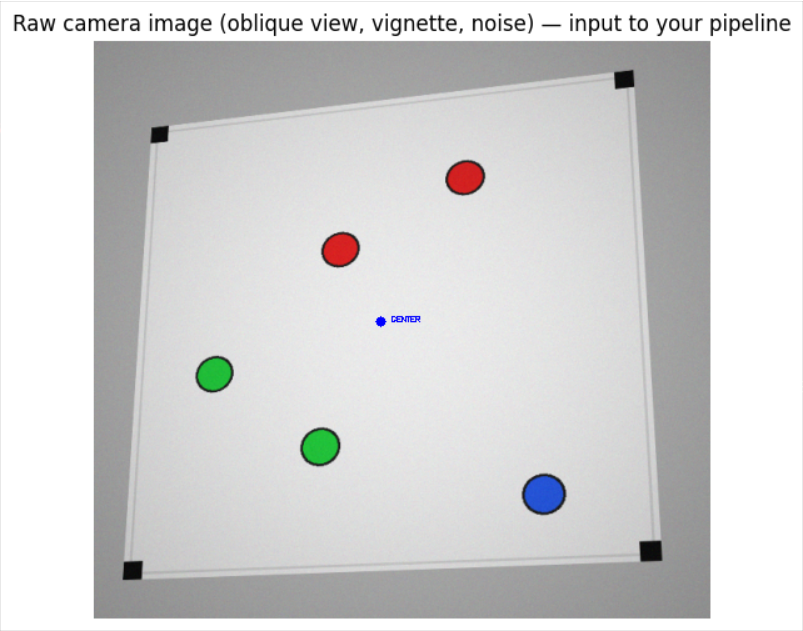
\includegraphics[width=\linewidth]{ogCenter.png}
    \caption{مرکز نشانگرها در تصویر قبل از \lr{warp} کردن پرسپکتیو}
    \label{fig:a}
  \end{minipage}\hfill
  \begin{minipage}{0.49\textwidth}
    \centering
    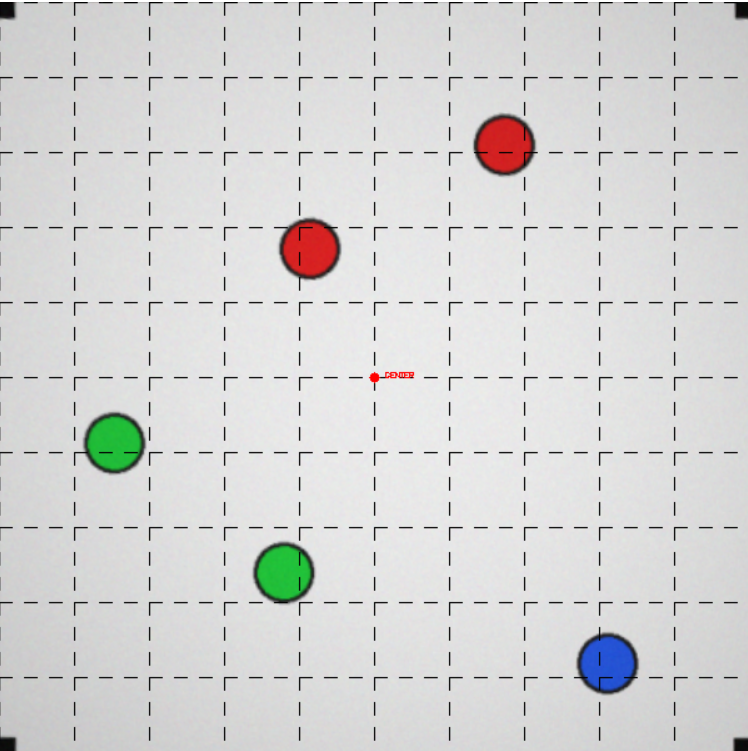
\includegraphics[width=\linewidth]{newCenter.png}
    \caption{مرکز نشانگرها در تصویر بعد از \lr{warp} کردن پرسپکتیو}
    \label{fig:b}
  \end{minipage}
\end{figure}

\subsubsection{تسک \lr{A.4} --- بخش‌بندی و پیدا کردن دیسک‌ها در فضای \lr{HSV}}

در این تسک، روی تصویر اصلاح شده مرحله قبل، دیسک‌های قرمز، آبی و سبز را پیدا کرده و همچنین مختصات مرکز \lr{(Centroid)} هر کدام را استخراج می‌کنیم. 

\subsubsection*{چالش‌های این مرحله}
\paragraph{1. رنگ قرمز در فضای \lr{HSV}:}\mbox{}\\
در فضای رنگی \lr{HSV}، مولفه \lr{Hue} در یک دایره 360 درجه تعریف می‌شود. رنگ‌های آبی و سبز در نواحی میانی این دایره قرار دارند و با یک بازه پیوسته تعریف می‌شوند. اما رنگ قرمز در ابتدا و انتهای دایره قرار دارد \lr{(Wrap-around)}. بنابراین برای شناسایی کامل طیف قرمز، باید دو بازه مجزا تعریف کرده و حاصل‌های به دست آمده را با عملگر \lr{OR} ترکیب کنیم.
\paragraph{2. اثر تیرگی و سایه روشن لنز پس از اصلاح تصویر}\mbox{}\\
اثر تیرگی گوشه‌های لنز باعث کاهش روشنایی در لبه‌های تصویر شده و سایه‌ها باعث تغییر فام (در فضای \lr{RGB}) می‌گردند. استفاده از فضای \lr{HSV} تا حدی مقاومت ایجاد می‌کند، اما کافی نیست. بنابراین برای حذف نویزهای کوچک با تعریف یک مساحت حداقلی، یک فیلتر روی مساحت اشیاء پیدا شده اعمال می‌کنیم.

\paragraph{3. احتمال به هم چسبیده بودن دیسک‌های هم‌رنگ}\mbox{}\\
ممکن است در تصویر دو دیسک هم‌رنگ، چسبیده به هم قرار گرفته باشند. بنابراین نباید کل پیکسل‌های یک رنگ، یک شیء واحد در نظر گرفته شوند. 
الگوریتم \lr{Connected-Component Analysis} هر ناحیه پیوسته را برچسب‌ \lr{Label} می‌زند و برای تفکیک آن‌ها می‌توان از عملیات‌های مورفولوژیک \mintinline{python}{cv2.morphologyEx} استفاده کرد، تا هر دیسک به درستی و مجرا شمرده شود. 


\paragraph{کد پیاده‌سازی شده}\mbox{}\\
کد این بخش در قسمت زیر قابل مشاهده است:
\addcontentsline{lol}{lstlisting}{کد تسک \lr{A.4}}
\begin{latin}
\begin{LTR}
\begin{minted}{python}
import cv2
import numpy as np

def segment_discs_and_show(path_to_png):
    """
    Load HSV image from file, segment colored discs, separate touching components.
    Show results and return list of (color_name, u, v) in pixel coordinates.
    """
    # read a3
    rectified_img = cv2.imread(path_to_png, cv2.IMREAD_COLOR)
    if rectified_img is None:
        raise FileNotFoundError(f"Cannot load image: {path_to_png}")

    hsv = cv2.cvtColor(rectified_img, cv2.COLOR_BGR2HSV)
    results = []

    # blue & green: 1 range/ red: 2 ranges
    color_ranges = {
        'red': [
            ([0,   100, 100], [10,  255, 255]),   # low red
            ([170, 100, 100], [180, 255, 255])    # high red
        ],
        'green': [
            ([40,  80,  80],  [80,  255, 255])
        ],
        'blue': [
            ([100, 80, 80],   [130, 255, 255])
        ],
    }


    # kernels morphological separation

    open_kernel      = cv2.getStructuringElement(cv2.MORPH_ELLIPSE, (5, 5))
    close_kernel     = cv2.getStructuringElement(cv2.MORPH_ELLIPSE, (9, 9))
    separate_kernel  = cv2.getStructuringElement(cv2.MORPH_ELLIPSE, (11, 11))

    # copy of original
    vis_img = rectified_img.copy()

    # process each color 
    for color_name, ranges in color_ranges.items():

        # combine masks for red
        mask = np.zeros(hsv.shape[:2], dtype=np.uint8)
        for lo, hi in ranges:
            lo = np.array(lo, dtype=np.uint8)
            hi = np.array(hi, dtype=np.uint8)
            mask |= cv2.inRange(hsv, lo, hi)

        # morphological separation
        mask = cv2.morphologyEx(mask, cv2.MORPH_OPEN,  open_kernel)
        mask = cv2.morphologyEx(mask, cv2.MORPH_CLOSE, close_kernel)
        mask = cv2.morphologyEx(mask, cv2.MORPH_OPEN,  separate_kernel)

        # connected components
        n_labels, labels, stats, centroids = cv2.connectedComponentsWithStats(
            mask, connectivity=8
        )

        # random color for components (displayed only)
        # shows separate images for separate disks on black background
        comp_vis = np.zeros((mask.shape[0], mask.shape[1], 3), dtype=np.uint8)
        rng = np.random.default_rng(42)

        for label in range(1, n_labels):  # skip background
            area = stats[label, cv2.CC_STAT_AREA]
            if area < 400:  # for small noise
                continue

            # centroid
            cx, cy = centroids[label]
            u = int(round(cx))
            v = int(round(cy))

            # store results
            results.append((color_name, u, v))

            # draw centroid
            cv2.circle(vis_img, (u, v), 4, (0, 0, 255), -1)
            cv2.putText(
                vis_img,
                f"{color_name}",
                (u + 5, v - 5),
                cv2.FONT_HERSHEY_SIMPLEX,
                0.4,
                (0, 0, 255),
                1
            )

            color = rng.integers(50, 255, size=3, dtype=np.uint8)
            comp_vis[labels == label] = color

        # show per color imgs
        cv2.imshow(f"{color_name} components (separated)", comp_vis)

    # final
    cv2.imshow("Original with centroids", vis_img)

    # tupple out
    tuple_output = [(color, (u, v)) for (color, u, v) in results]
    print("Detected discs (color, (u, v)):")
    for t in tuple_output:
        print(t)

    cv2.waitKey(0)
    cv2.destroyAllWindows()

    return tuple_output


# run
path_to_png = r"C:\Users\Asus\Desktop\hasti\a3.png"   # edit this as needed
results = segment_discs_and_show(path_to_png)

\end{minted}
\end{LTR}
\end{latin}

\paragraph{خروجی کد}\mbox{}\\
در کد این بخش، علاوه بر مشخص کردن دیسک‌ها بر روی خروجی مرحله قبلی (شکل \ref{fig:b}) که در شکل \ref{fig:all} قابل مشاهده است، دیسک‌ها را به صورت تفکیک‌شده بر اساس رنگ، در تصویرهای مستقل نمایش داده‌ایم که در شکل \ref{fig:sep} قابل مشاهده هستند.
\begin{figure}[H]
    \centering
    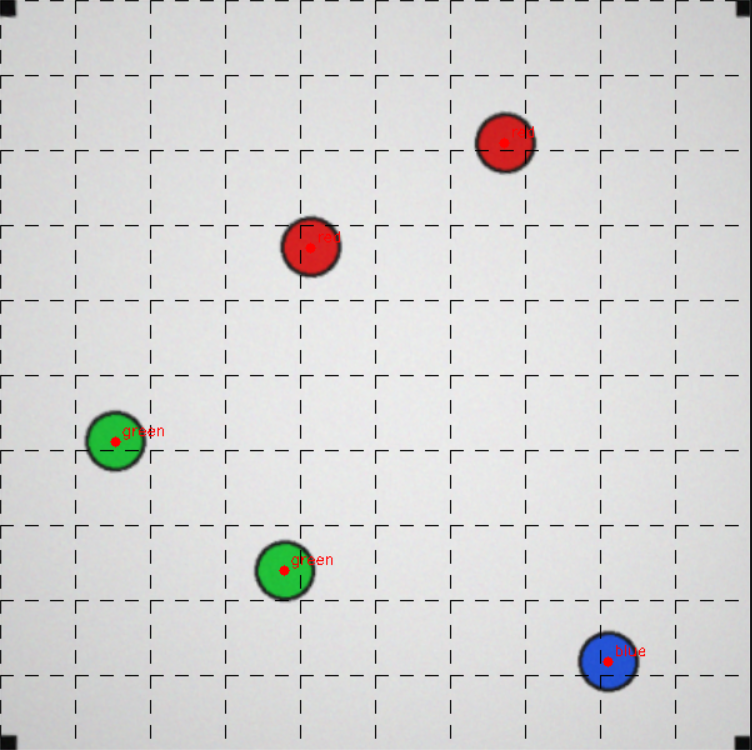
\includegraphics[width=0.8\textwidth, keepaspectratio]{allseg.png}
    \caption{مشخص کردن نشانگرها روی تصویر به ترتیب ساعتگرد}
    \label{fig:all}
\end{figure}

\begin{figure}[htbp]
     \centering
     % First Subfigure
     \begin{subfigure}[b]{0.3\textwidth}
         \centering
         
\includegraphics[width=\textwidth]{BC.png}
         \caption{دیسک آبی}
         \label{fig:sep1}
     \end{subfigure}
     \hfill
     % Second Subfigure
     \begin{subfigure}[b]{0.3\textwidth}
         \centering
         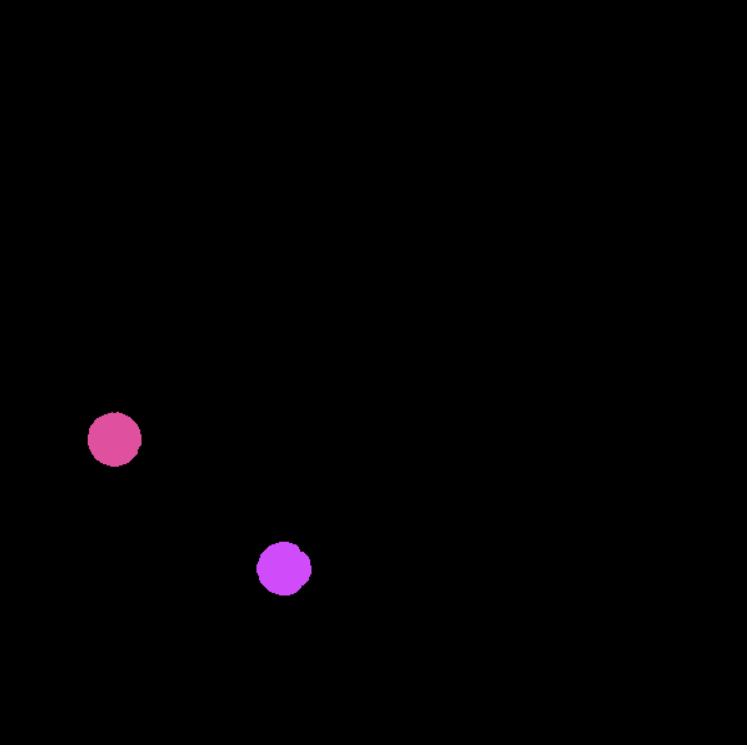
\includegraphics[width=\textwidth]{GC.png}
         \caption{دیسک‌های سبز}
         \label{fig:sep2}
     \end{subfigure}
     \hfill
     % Third Subfigure
     \begin{subfigure}[b]{0.3\textwidth}
         \centering
         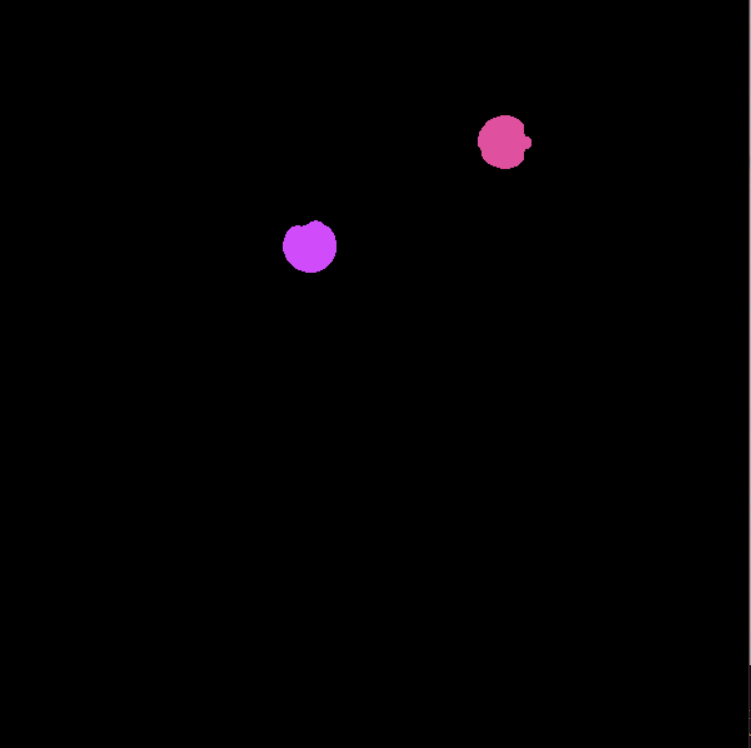
\includegraphics[width=\textwidth]{RC.png}
         \caption{دیسک‌های قرمز}
         \label{fig:sep3}
     \end{subfigure}
     
     \caption{تصویرهای مستقل از دیسک‌ها با تفکیک بر اساس رنگ}
     \label{fig:sep}
\end{figure}

علاوه بر این تصاویر، مختصات مرکز ثقل دیسک‌ها نیز به صورت \lr{Tupple} خروجی دیگر این کد است:
\begin{latin}
\begin{LTR}
\begin{verbatim}
Detected corners:
[[127. 106.]
 [498.  62.]
 [520. 439.]
 [105. 455.]]
Detected discs (color, (u, v)):
('red', (403, 114))
('red', (248, 198))
('green', (92, 353))
('green', (227, 456))
('blue', (486, 529))
\end{verbatim}
\end{LTR}
\end{latin}

\subsubsection{تسک \lr{A.5} --- تبدیل مختصات به دستگاه ربات و تکمیل نهایی پایپ لاین}
در گام آخر، مختصات پیکسلی مرکز هر دیسک را با استفاده تناسب تعریف شده در مرحله قبل به مختصات واقعی و متریک تیدیل می‌کنیم. سپس تمام توابع نوشته شده در تسک‌های پیشین را در یک تابع به نام \mintinline{python}{vision_pipeline} تجمیع کرده و مختصات محاسبه شده را با مختصات واقعی قطعات \lr{(Ground-truth)} مقایسه کرده و خطای الگوریتم بینایی را به دست می‌آوریم.



\paragraph{به دست آوردن مختصات واقعی و خطای الگوریتم بینایی}\mbox{}\\
با توجه به این که هر یک متر در دنیای واقعی برابر با 1000 پیکسل در نظر گرفته شده است، با استفاده از تابع زیر، مختصات واقعی مرکز ثقل دیسک‌ها را به دست می‌آوریم:

\begin{latin}
\begin{LTR}
\begin{listing}[htbp]
\begin{minted}{python}
def world_to_pixel(world_x, world_y, center_u=300, center_v=300, scale=1000):
    u = int(center_u - world_y * scale)
    v = int(center_v - world_x * scale)
    return (u, v)
\end{minted}
\end{listing}
\end{LTR}
\end{latin}



خروجی این تابع 

\begin{latin}
\begin{LTR}
\begin{verbatim}
  red: pixel (404, 114) -> world (+0.186, -0.104)
  red: pixel (248, 197) -> world (+0.103, +0.052)
  green: pixel (92, 353) -> world (-0.053, +0.208)
  green: pixel (228, 456) -> world (-0.156, +0.072)
  blue: pixel (486, 529) -> world (-0.229, -0.186)
\end{verbatim}
\end{LTR}
\end{latin}
است.

سپس با تابع دیگری که در زیر تعریف شده، این مختصات را با مختصات \lr{Ground Truth} مقایسه می‌کنیم و خطای الگوریتم بینایی را به دست می‌آوریم:

\begin{latin}
\begin{LTR}
\begin{listing}[htbp]
\begin{minted}{python}
def match_discs_to_ground_truth(detected_discs, ground_truth):
    detected_world = [
        {"color": color, "world_xy": pixel_to_world(u, v), "pixel_uv": (u, v)}
        for color, u, v in detected_discs
    ]
    
    gt_remaining = ground_truth.copy()
    matches = []
    
    for det in detected_world:
        best_match = None
        best_distance = float('inf')
        
        for gt in gt_remaining:
            if gt["color"] != det["color"]:
                continue
            
            dx = det["world_xy"][0] - gt["world_xy"][0]
            dy = det["world_xy"][1] - gt["world_xy"][1]
            distance = np.sqrt(dx**2 + dy**2)
            
            if distance < best_distance:
                best_distance = distance
                best_match = gt
        
        if best_match:
            error_x = det["world_xy"][0] - best_match["world_xy"][0]
            error_y = det["world_xy"][1] - best_match["world_xy"][1]
            
            matches.append({
                "color": det["color"],
                "detected_world_xy": det["world_xy"],
                "detected_pixel_uv": det["pixel_uv"],
                "ground_truth_world_xy": best_match["world_xy"],
                "error_xy": (error_x, error_y),
                "error_magnitude": best_distance
            })
            
            gt_remaining.remove(best_match)
    
    return matches, gt_remaining
\end{minted}
\end{listing}
\end{LTR}
\end{latin}

خروجی این تابع به صورت جدول با دقت میلی‌متر در پایین قابل مشاهده است.
\begin{latin}
\begin{LTR}
\begin{verbatim}
--------------------------------------------------------------------------------
Color    Detected (world)     Ground Truth         Error                Magnitude 
--------------------------------------------------------------------------------
red      (+0.186, -0.104)     (+0.180, -0.100)     (+0.006, -0.004)     0.0072    
red      (+0.103, +0.052)     (+0.100, +0.050)     (+0.003, +0.002)     0.0036    
green    (-0.053, +0.208)     (-0.050, +0.200)     (-0.003, +0.008)     0.0085    
green    (-0.156, +0.072)     (-0.150, +0.070)     (-0.006, +0.002)     0.0063    
blue     (-0.229, -0.186)     (-0.220, -0.180)     (-0.009, -0.006)     0.0108    
\end{verbatim}
\end{LTR}
\end{latin}


\paragraph{تجمیع توابع}\mbox{}\\
با تجمیع همه توابع نوشته شده در تسک‌های پیشین و اضافه کردن دو تابع دیگر برای بدست آوردن مختصات واقعی و همچنین پیدا کردن خطا، در نهایت پایپ‌لاین کامل به صورت زیر پیاده‌سازی می‌شود:
\addcontentsline{lol}{lstlisting}{کد تسک \lr{A.5}}
\begin{latin}
\begin{LTR}
\begin{minted}{python}
import cv2
import numpy as np
from pathlib import Path


GROUND_TRUTH_DISCS = [
    {"color": "red",   "world_xy": (+0.18, -0.10)},
    {"color": "green", "world_xy": (-0.05, +0.20)},
    {"color": "blue",  "world_xy": (-0.22, -0.18)},
    {"color": "red",   "world_xy": (+0.10, +0.05)},
    {"color": "green", "world_xy": (-0.15, +0.07)},
]


def detect_corner_markers(image):
    hsv = cv2.cvtColor(image, cv2.COLOR_BGR2HSV)
    
    _, binary = cv2.threshold(
        hsv[:, :, 2],
        50,
        255,
        cv2.THRESH_BINARY_INV
    )
    
    contours, _ = cv2.findContours(
        binary,
        cv2.RETR_EXTERNAL,
        cv2.CHAIN_APPROX_SIMPLE
    )
    
    square_candidates = []
    
    for cnt in contours:
        area = cv2.contourArea(cnt)
        
        if area < 100:
            continue
        
        x, y, w, h = cv2.boundingRect(cnt)
        box_area = w * h
        squareness = area / box_area if box_area > 0 else 0
        
        if squareness > 0.3:
            square_candidates.append(cnt)
    
    square_candidates.sort(key=cv2.contourArea, reverse=True)
    top4 = square_candidates[:4]
    
    centers = []
    for cnt in top4:
        M = cv2.moments(cnt)
        
        if M['m00'] == 0:
            continue
        
        cx = int(M['m10'] / M['m00'])
        cy = int(M['m01'] / M['m00'])
        centers.append((cx, cy))
    
    centers = sort_clockwise(centers)
    return np.float32(centers)


def sort_clockwise(pts):
    pts = sorted(pts, key=lambda p: p[1])
    top = sorted(pts[:2], key=lambda p: p[0])
    bottom = sorted(pts[2:], key=lambda p: p[0], reverse=True)
    return [top[0], top[1], bottom[0], bottom[1]]


def compute_center(corners):
    p1, p2, p3, p4 = corners[0], corners[2], corners[1], corners[3]
    
    x1, y1 = p1.astype(np.float64)
    x2, y2 = p2.astype(np.float64)
    x3, y3 = p3.astype(np.float64)
    x4, y4 = p4.astype(np.float64)
    
    A1 = y2 - y1
    B1 = x1 - x2
    C1 = A1 * x1 + B1 * y1
    
    A2 = y4 - y3
    B2 = x3 - x4
    C2 = A2 * x3 + B2 * y3
    
    det = A1 * B2 - A2 * B1
    
    center_x = (B2 * C1 - B1 * C2) / det
    center_y = (A1 * C2 - A2 * C1) / det
    
    return np.array([[[center_x, center_y]]], dtype=np.float32)


def rectify_image(image, corners, canvas_size=600):
    dst_points = np.float32([
        [0, 0],
        [canvas_size - 1, 0],
        [canvas_size - 1, canvas_size - 1],
        [0, canvas_size - 1]
    ])
    
    H, _ = cv2.findHomography(corners, dst_points)
    
    rectified = cv2.warpPerspective(
        image,
        H,
        (canvas_size, canvas_size)
    )
    
    return rectified, H


def draw_grid(image, canvas_size=600, grid_spacing=60, dash_length=10, gap_length=10):
    result = image.copy()
    
    for x in range(0, canvas_size, grid_spacing):
        y = 0
        while y < canvas_size:
            y_end = min(y + dash_length, canvas_size)
            cv2.line(result, (x, y), (x, y_end), (0, 0, 0), 1)
            y += dash_length + gap_length
    
    for y in range(0, canvas_size, grid_spacing):
        x = 0
        while x < canvas_size:
            x_end = min(x + dash_length, canvas_size)
            cv2.line(result, (x, y), (x_end, y), (0, 0, 0), 1)
            x += dash_length + gap_length
    
    return result


def segment_discs(rectified_img):
    hsv = cv2.cvtColor(rectified_img, cv2.COLOR_BGR2HSV)
    results = []
    
    color_ranges = {
        'red': [
            ([0,   100, 100], [10,  255, 255]),
            ([170, 100, 100], [180, 255, 255])
        ],
        'green': [
            ([40,  80,  80],  [80,  255, 255])
        ],
        'blue': [
            ([100, 80, 80],   [130, 255, 255])
        ],
    }
    
    open_kernel = cv2.getStructuringElement(cv2.MORPH_ELLIPSE, (5, 5))
    close_kernel = cv2.getStructuringElement(cv2.MORPH_ELLIPSE, (9, 9))
    separate_kernel = cv2.getStructuringElement(cv2.MORPH_ELLIPSE, (11, 11))
    
    for color_name, ranges in color_ranges.items():
        mask = np.zeros(hsv.shape[:2], dtype=np.uint8)
        
        for lo, hi in ranges:
            lo = np.array(lo, dtype=np.uint8)
            hi = np.array(hi, dtype=np.uint8)
            mask |= cv2.inRange(hsv, lo, hi)
        
        mask = cv2.morphologyEx(mask, cv2.MORPH_OPEN, open_kernel)
        mask = cv2.morphologyEx(mask, cv2.MORPH_CLOSE, close_kernel)
        mask = cv2.morphologyEx(mask, cv2.MORPH_OPEN, separate_kernel)
        
        n_labels, labels, stats, centroids = cv2.connectedComponentsWithStats(
            mask, connectivity=8
        )
        
        for label in range(1, n_labels):
            area = stats[label, cv2.CC_STAT_AREA]
            if area < 400:
                continue
            
            cx, cy = centroids[label]
            u = int(round(cx))
            v = int(round(cy))
            
            results.append((color_name, u, v))
    
    return results


def pixel_to_world(u, v, center_u=300, center_v=300, scale=1000):
    world_x = (center_v - v) / scale
    world_y = (center_u - u) / scale
    return (world_x, world_y)


def world_to_pixel(world_x, world_y, center_u=300, center_v=300, scale=1000):
    u = int(center_u - world_y * scale)
    v = int(center_v - world_x * scale)
    return (u, v)


def match_discs_to_ground_truth(detected_discs, ground_truth):
    detected_world = [
        {"color": color, "world_xy": pixel_to_world(u, v), "pixel_uv": (u, v)}
        for color, u, v in detected_discs
    ]
    
    gt_remaining = ground_truth.copy()
    matches = []
    
    for det in detected_world:
        best_match = None
        best_distance = float('inf')
        
        for gt in gt_remaining:
            if gt["color"] != det["color"]:
                continue
            
            dx = det["world_xy"][0] - gt["world_xy"][0]
            dy = det["world_xy"][1] - gt["world_xy"][1]
            distance = np.sqrt(dx**2 + dy**2)
            
            if distance < best_distance:
                best_distance = distance
                best_match = gt
        
        if best_match:
            error_x = det["world_xy"][0] - best_match["world_xy"][0]
            error_y = det["world_xy"][1] - best_match["world_xy"][1]
            
            matches.append({
                "color": det["color"],
                "detected_world_xy": det["world_xy"],
                "detected_pixel_uv": det["pixel_uv"],
                "ground_truth_world_xy": best_match["world_xy"],
                "error_xy": (error_x, error_y),
                "error_magnitude": best_distance
            })
            
            gt_remaining.remove(best_match)
    
    return matches, gt_remaining


def vision_pipeline(image_path, output_dir="./output", canvas_size=600, 
                   grid_spacing=60, visualize=True):
    output_dir = Path(output_dir)
    output_dir.mkdir(exist_ok=True)
    
    image = cv2.imread(str(image_path))
    
    print("="*60)
    print("VISION PIPELINE")
    print("="*60)
    
    print("\nStep 1: Detecting corner markers...")
    corners = detect_corner_markers(image)
    print(f"Detected corners:\n{corners}")
    
    print("\nStep 2: Computing center and rectifying...")
    center_original = compute_center(corners)
    rectified_image, homography = rectify_image(image, corners, canvas_size)
    center_rectified = cv2.perspectiveTransform(center_original, homography)
    
    cx_orig = int(round(center_original[0][0][0]))
    cy_orig = int(round(center_original[0][0][1]))
    cx_rect = int(round(center_rectified[0][0][0]))
    cy_rect = int(round(center_rectified[0][0][1]))
    
    print(f"Original center: ({cx_orig}, {cy_orig})")
    print(f"Rectified center: ({cx_rect}, {cy_rect})")
    
    print("\nCorner world coordinates:")
    corner_labels = ["Top-Left", "Top-Right", "Bottom-Right", "Bottom-Left"]
    expected_coords = [(0.3, 0.3), (0.3, -0.3), (-0.3, -0.3), (-0.3, 0.3)]
    for i, (label, expected) in enumerate(zip(corner_labels, expected_coords)):
        u, v = 0 if i % 2 == 0 else canvas_size - 1, 0 if i < 2 else canvas_size - 1
        world_x, world_y = pixel_to_world(u, v)
        print(f"  {label}: pixel ({u}, {v}) -> world ({world_x:+.3f}, {world_y:+.3f}) [expected: {expected}]")
    
    rectified_with_grid = draw_grid(rectified_image, canvas_size, grid_spacing)
    
    print("\nStep 3: Segmenting colored discs...")
    detected_discs = segment_discs(rectified_image)
    
    print(f"\nDetected {len(detected_discs)} discs (pixel coordinates):")
    for color, u, v in detected_discs:
        print(f"  {color}: ({u}, {v})")
    
    print("\nStep 4: Converting to world coordinates...")
    discs_world = []
    for color, u, v in detected_discs:
        world_x, world_y = pixel_to_world(u, v)
        discs_world.append({
            "color": color,
            "pixel_uv": (u, v),
            "world_xy": (world_x, world_y)
        })
        print(f"  {color}: pixel ({u}, {v}) -> world ({world_x:+.3f}, {world_y:+.3f})")
    
    print("\nStep 5: Comparing with ground truth...")
    matches, unmatched_gt = match_discs_to_ground_truth(detected_discs, GROUND_TRUTH_DISCS)
    
    print(f"\nMatched {len(matches)} discs:")
    print("\n" + "-"*80)
    print(f"{'Color':<8} {'Detected (world)':<20} {'Ground Truth':<20} {'Error':<20} {'Magnitude':<10}")
    print("-"*80)
    
    for match in matches:
        det_str = f"({match['detected_world_xy'][0]:+.3f}, {match['detected_world_xy'][1]:+.3f})"
        gt_str = f"({match['ground_truth_world_xy'][0]:+.3f}, {match['ground_truth_world_xy'][1]:+.3f})"
        err_str = f"({match['error_xy'][0]:+.3f}, {match['error_xy'][1]:+.3f})"
        mag_str = f"{match['error_magnitude']:.4f}"
        
        print(f"{match['color']:<8} {det_str:<20} {gt_str:<20} {err_str:<20} {mag_str:<10}")
    
    if unmatched_gt:
        print(f"\nUnmatched ground truth discs: {len(unmatched_gt)}")
        for gt in unmatched_gt:
            print(f"  {gt['color']}: {gt['world_xy']}")
    
    if visualize:
        vis_corners = image.copy()
        labels = ["TL", "TR", "BR", "BL"]
        for i, (x, y) in enumerate(corners.astype(int)):
            cv2.circle(vis_corners, (x, y), 10, (0, 0, 255), -1)
            cv2.putText(vis_corners, labels[i], (x + 10, y - 10),
                       cv2.FONT_HERSHEY_SIMPLEX, 0.7, (0, 255, 0), 2)
        
        vis_center = image.copy()
        cv2.circle(vis_center, (cx_orig, cy_orig), 4, (255, 0, 0), -1)
        cv2.putText(vis_center, "CENTER", (cx_orig + 8, cy_orig),
                   cv2.FONT_HERSHEY_SIMPLEX, 0.2, (255, 0, 0), 1)
        
        vis_rectified = rectified_with_grid.copy()
        cv2.circle(vis_rectified, (cx_rect, cy_rect), 4, (0, 0, 255), -1)
        cv2.putText(vis_rectified, "CENTER", (cx_rect + 8, cy_rect),
                   cv2.FONT_HERSHEY_SIMPLEX, 0.2, (0, 0, 255), 1)
        
        vis_discs = rectified_image.copy()
        for color, u, v in detected_discs:
            cv2.circle(vis_discs, (u, v), 4, (0, 0, 255), -1)
            cv2.putText(vis_discs, color, (u + 5, v - 5),
                       cv2.FONT_HERSHEY_SIMPLEX, 0.4, (0, 0, 255), 1)
        
        vis_comparison = rectified_image.copy()
        
        cv2.circle(vis_comparison, (300, 300), 5, (128, 128, 128), -1)
        
        for gt in GROUND_TRUTH_DISCS:
            gt_u, gt_v = world_to_pixel(gt["world_xy"][0], gt["world_xy"][1])
            cv2.circle(vis_comparison, (gt_u, gt_v), 8, (0, 255, 0), 2)
            cv2.putText(vis_comparison, f"GT-{gt['color']}", (gt_u + 10, gt_v - 10),
                       cv2.FONT_HERSHEY_SIMPLEX, 0.3, (0, 255, 0), 1)
        
        for match in matches:
            det_u, det_v = match['detected_pixel_uv']
            gt_u, gt_v = world_to_pixel(match['ground_truth_world_xy'][0], 
                                        match['ground_truth_world_xy'][1])
            
            cv2.circle(vis_comparison, (det_u, det_v), 6, (0, 0, 255), -1)
            cv2.line(vis_comparison, (det_u, det_v), (gt_u, gt_v), (255, 0, 255), 1)
            
            mid_u = (det_u + gt_u) // 2
            mid_v = (det_v + gt_v) // 2
            cv2.putText(vis_comparison, f"{match['error_magnitude']:.3f}", 
                       (mid_u, mid_v), cv2.FONT_HERSHEY_SIMPLEX, 0.3, (255, 0, 255), 1)
        
        cv2.imwrite(str(output_dir / "1_detected_corners.jpg"), vis_corners)
        cv2.imwrite(str(output_dir / "2_original_center.jpg"), vis_center)
        cv2.imwrite(str(output_dir / "3_rectified_grid.jpg"), vis_rectified)
        cv2.imwrite(str(output_dir / "4_segmented_discs.jpg"), vis_discs)
        cv2.imwrite(str(output_dir / "5_error_comparison.jpg"), vis_comparison)
        cv2.imwrite(str(output_dir / "rectified.png"), rectified_image)
        
        print(f"\nVisualizations saved to {output_dir}/")
    
    errors_x = [m['error_xy'][0] for m in matches]
    errors_y = [m['error_xy'][1] for m in matches]
    errors_mag = [m['error_magnitude'] for m in matches]
    
    return {
        'corners': corners,
        'center_original': (cx_orig, cy_orig),
        'center_rectified': (cx_rect, cy_rect),
        'homography': homography,
        'rectified_image': rectified_image,
        'detected_discs_pixel': [(color, (u, v)) for color, u, v in detected_discs],
        'detected_discs_world': discs_world,
        'matches': matches,
        'unmatched_ground_truth': unmatched_gt,
        'error_statistics': {
            'mean_error_x': np.mean(errors_x) if matches else None,
            'mean_error_y': np.mean(errors_y) if matches else None,
            'rms_error_x': np.sqrt(np.mean(np.array(errors_x)**2)) if matches else None,
            'rms_error_y': np.sqrt(np.mean(np.array(errors_y)**2)) if matches else None,
            'mean_magnitude': np.mean(errors_mag) if matches else None,
            'max_magnitude': np.max(errors_mag) if matches else None,
        }
    }


if __name__ == "__main__":
    image_path = r"C:\Users\Asus\Desktop\hasti\output.png"
    
    results = vision_pipeline(
        image_path=image_path,
        output_dir="./output",
        canvas_size=600,
        grid_spacing=60,
        visualize=True
    )
    
    print("\n" + "="*60)
    print("PIPELINE COMPLETE")
    print("="*60)

\end{minted}
\end{LTR}
\end{latin}
که خروجی آن به صورت زیر است:
\begin{latin}
\begin{LTR}
\begin{verbatim}
============================================================
VISION PIPELINE
============================================================

Step 1: Detecting corner markers...
Detected corners:
[[ 49.  72.]
 [420.  28.]
 [442. 405.]
 [ 27. 421.]]

Step 2: Computing center and rectifying...
Original center: (226, 222)
Rectified center: (300, 300)

Corner world coordinates:
  Top-Left: pixel (0, 0) -> world (+0.300, +0.300) [expected: (0.3, 0.3)]
  Top-Right: pixel (599, 0) -> world (+0.300, -0.299) [expected: (0.3, -0.3)]
  Bottom-Right: pixel (0, 599) -> world (-0.299, +0.300) [expected: (-0.3, -0.3)]
  Bottom-Left: pixel (599, 599) -> world (-0.299, -0.299) [expected: (-0.3, 0.3)]

Step 3: Segmenting colored discs...

Detected 5 discs (pixel coordinates):
  red: (404, 114)
  red: (248, 197)
  green: (92, 353)
  green: (228, 456)
  blue: (486, 529)

Step 4: Converting to world coordinates...
  red: pixel (404, 114) -> world (+0.186, -0.104)
  red: pixel (248, 197) -> world (+0.103, +0.052)
  green: pixel (92, 353) -> world (-0.053, +0.208)
  green: pixel (228, 456) -> world (-0.156, +0.072)
  blue: pixel (486, 529) -> world (-0.229, -0.186)

Step 5: Comparing with ground truth...

Matched 5 discs:

--------------------------------------------------------------------------------
Color    Detected (world)     Ground Truth         Error                Magnitude 
--------------------------------------------------------------------------------
red      (+0.186, -0.104)     (+0.180, -0.100)     (+0.006, -0.004)     0.0072    
red      (+0.103, +0.052)     (+0.100, +0.050)     (+0.003, +0.002)     0.0036    
green    (-0.053, +0.208)     (-0.050, +0.200)     (-0.003, +0.008)     0.0085    
green    (-0.156, +0.072)     (-0.150, +0.070)     (-0.006, +0.002)     0.0063    
blue     (-0.229, -0.186)     (-0.220, -0.180)     (-0.009, -0.006)     0.0108    

Visualizations saved to output/

============================================================
PIPELINE COMPLETE
============================================================
\end{verbatim}
\end{LTR}
\end{latin}

\subsection{بخش \lr{B} --- سینماتیک مستقیم \lr{(Forward Kinematics)} ربات \lr{PRR}}

\paragraph{معرفی ربات و ساختار کلی آن}\mbox{}\\
ربات مورد بررسی یک ربات بازرس از نوع PRR است که از سه مفصل تشکیل شده است. حرف P نشان‌دهنده یک مفصل منشوری (کشویی) و دو حرف R نشان‌دهنده دو مفصل لولایی (دورانی) می‌باشند. ساختار این ربات به گونه‌ای است که مفصل اول وظیفه تنظیم ارتفاع کل بازو را بر عهده دارد و دو مفصل بعدی، مانند یک بازوی صفحه‌ای \lr{(Planar)}، در یک صفحه افقی حرکت می‌کنند تا به نقطه هدف برسند.  

\paragraph{مشخصات مفاصل و پارامترهای فیزیکی}\mbox{}\\
بر اساس اطلاعات موجود، پارامترهای حرکتی و ابعاد فیزیکی ربات به شرح زیر است:
\begin{itemize}
	\item \textbf{مفصل ۱ (کشویی):} این مفصل در امتداد محور $Z$ جهانی حرکت می‌کند. دامنه حرکتی آن $q_1 \in [0, 0.50]$ متر است. ارتفاع اولیه محور مفصل دوم از سطح زمین برابر با $D_0 = 0.70$ متر می‌باشد.
	\item \textbf{مفصل ۲ (دورانی):} این مفصل حول محور $Z$ دوران می‌کند و قابلیت چرخش کامل به صورت $q_2 \in [-\pi, +\pi]$ را دارد. طول لینک آن $L_2 = 0.40$ متر است.
	\item \textbf{مفصل ۳ (دورانی):} این مفصل نیز حول محور $Z$ می‌چرخد و دامنه حرکتی آن $q_3 \in [-\pi, +\pi]$   است. طول لینک آن  $L_3 = 0.30$ متر می‌باشد .
\end{itemize}
نقطه ابزار (افکتور نهایی) در محل تقاطع محور دورانی سوم با نوک لینک آخر قرار دارد و طول ابزار متصل به آن صفر در نظر گرفته شده است.

\subsubsection{تسک \lr{B.1} -- جدول پارامترهای دناویت-هاروتنبرگ (DH)}

با استفاده از روش استاندارد \lr{DH}، جدول پارامترهای این ربات به شکل زیر تدوین می‌شود (متغیرهای مفصلی به صورت پررنگ مشخص شده‌اند):

\begin{table}[htbp]
	\centering
	\renewcommand{\arraystretch}{1.5}
	\begin{tabular}{|c|c|c|c|c|c|}
		\hline
		\textbf{لینک $i$} & $\alpha_{i-1}$ \textbf{(رادیان)} & $a_{i-1}$ \textbf{(متر)} & $d_i$ \textbf{(متر)} & $\theta_i$ \textbf{(رادیان)} & \textbf{نوع مفصل} \\ \hline
		۱ & 0 & 0 & $\mathbf{D_0 + q_1}$ & 0 & کشویی (P) \\ \hline
		۲ & 0 & $L_2$ & 0 & $\mathbf{q_2}$ & دورانی (R) \\ \hline
		۳ & 0 & $L_3$ & 0 & $\mathbf{q_3}$ & دورانی (R) \\ \hline
	\end{tabular}
\end{table}

هر سطر از این جدول برای ساخت ماتریس تبدیل مربوط به همان لینک استفاده می‌شود. فرمول کلی ساخت ماتریس انتقال در این روش به صورت ضرب چهار ماتریس پایه زیر است:
$$ ^{i-1}T_i = R_z(\theta_i) T_z(d_i) T_x(a_{i-1}) R_x(\alpha_{i-1}) $$

\paragraph{نحوه کارکرد و تحلیل حرکتی}\mbox{}\\
از نظر سینماتیکی، موقعیت نهایی ربات ترکیبی از این سه حرکت است. مفصل اول با تغییر متغیر $q_1$، مختصات ارتفاع (محور $Z$) نقطه نهایی را مستقیماً تعیین می‌کند. از آنجایی که $\alpha$ در تمامی مفاصل صفر است، صفحات حرکتی مفاصل دوم و سوم موازی با صفحه افقی ($XY$) باقی می‌مانند. مفاصل دوم و سوم به ترتیب با زوایای $q_2$ و $q_3$ و با استفاده از طول بازوهای $L_2$ و $L_3$، موقعیت افکتور را در این صفحه افقی مشخص می‌کنند. با ضرب ماتریس‌های تبدیلِ حاصل از جدول بالا، می‌توان معادلات دقیق موقعیت $x$، $y$ و $z$ افکتور نهایی را بر حسب مقادیر مفصلی محاسبه نمود.
\subsubsection{تسک\lr{B.2} — محاسبات نمادین با \lr{SymPy}}
\paragraph{نحوه پیاده‌سازی کد و محاسبه ماتریس‌ها}\mbox{}\\
برای محاسبه سینماتیک مستقیم این ربات به صورت پارامتری، از کتابخانه قدرتمند \lr{SymPy} در زبان پایتون استفاده شده است. در ابتدا، متغیرهای مفصلی ($q_1, q_2, q_3$) و پارامترهای ثابت فیزیکی ($D_0, L_2, L_3$) به عنوان متغیرهای نمادین (Symbolic) تعریف شده‌اند. سپس تابعی به نام \lr{\texttt{dh\_matrix}} نوشته شده است که با دریافت چهار پارامتر استاندارد دناویت-هارتنبرگ ($\theta, d, a, \alpha$)، ماتریس تبدیل همگن $4 \times 4$ مربوطه را تولید می‌کند. 
بر اساس جدول DH، ماتریس تبدیل هر لینک به صورت مجزا ($T_1^0, T_2^1, T_3^2$) ساخته شده و در نهایت با ضرب متوالی آن‌ها ($T_1^0 \times T_2^1 \times T_3^2$)، ماتریس تبدیل نهایی $^0T_3$ به دست آمده است. در انتها با استفاده از دستور \lr{\texttt{sp.simplify}}، عبارات مثلثاتی ساده‌سازی شده و ستون چهارم ماتریس به عنوان مختصات استخراج گردیده است.

\paragraph{کد پایتون پیاده‌سازی‌شده}\mbox{}\\
کد استفاده شده برای این محاسبات به شرح زیر است:

\addcontentsline{lol}{lstlisting}{کد تسک \lr{B.2}}
\begin{latin}
\begin{LTR}
\begin{minted}{python}
     import sympy as sp
     
     # Initialize printing for pretty formatting in Jupyter Notebook
     sp.init_printing(use_latex='mathjax')
     
     # 1. Define symbolic variables
     q1, q2, q3 = sp.symbols('q1 q2 q3')
     D0, L2, L3 = sp.symbols('D0 L2 L3')
     
     # Define DH transformation matrix function
     def dh_matrix(theta, d, a, alpha):
     return sp.Matrix([
     [sp.cos(theta), -sp.sin(theta)*sp.cos(alpha),  sp.sin(theta)*sp.sin(alpha), a*sp.cos(theta)],
     [sp.sin(theta),  sp.cos(theta)*sp.cos(alpha), -sp.cos(theta)*sp.sin(alpha), a*sp.sin(theta)],
     [0,              sp.sin(alpha),                sp.cos(alpha),               d],
     [0,              0,                            0,                           1]
     ])
     
     # 2. Construct transformation matrices for each link based on the DH table
     T1_0 = dh_matrix(0, D0 + q1, 0, 0)
     T2_1 = dh_matrix(q2, 0, L2, 0)
     T3_2 = dh_matrix(q3, 0, L3, 0)
     
     # 3. Calculate final transformation matrix (0T3 = T1_0 * T2_1 * T3_2)
     T3_0 = T1_0 * T2_1 * T3_2
     T3_0_simplified = sp.simplify(T3_0)
     
     # 4. Extract position coordinates (x, y, z)
     x = T3_0_simplified[0, 3]
     y = T3_0_simplified[1, 3]
     z = T3_0_simplified[2, 3]
     
     # 5. Display results clearly
     print("--- Final Transformation Matrix (0T3) ---")
     display(T3_0_simplified)
     
     print("\n--- End-Effector Position Equations (Symbolic) ---")
     display(sp.Matrix([x, y, z]))
     
     # 6. Numerical substitution for specific link lengths
     constants = {D0: 0.70, L2: 0.40, L3: 0.30}
     x_num = x.subs(constants)
     y_num = y.subs(constants)
     z_num = z.subs(constants)
     
     print("\n--- End-Effector Position Equations (with given constants) ---")
     print(f"x = {x_num}")
     print(f"y = {y_num}")
     print(f"z = {z_num}")
\end{minted}
\end{LTR}
\end{latin}


\paragraph{خروجی‌های به‌دست‌آمده (ماتریس و معادلات موقعیت)}\mbox{}\\
با اجرای کد بالا، ماتریس تبدیل نهایی $^0T_3$ به شکل ساده‌شده زیر به دست می‌آید:
$$
^0T_3 = \begin{bmatrix}
	\cos(q_2 + q_3) & -\sin(q_2 + q_3) & 0 & L_2\cos(q_2) + L_3\cos(q_2 + q_3) \\
	\sin(q_2 + q_3) & \cos(q_2 + q_3) & 0 & L_2\sin(q_2) + L_3\sin(q_2 + q_3) \\
	0 & 0 & 1 & D_0 + q_1 \\
	0 & 0 & 0 & 1
\end{bmatrix}
$$

معادلات موقعیت مجری نهایی (End-Effector) به صورت نمادین:
$$ x = L_2 \cos(q_2) + L_3 \cos(q_2 + q_3) $$
$$ y = L_2 \sin(q_2) + L_3 \sin(q_2 + q_3) $$
$$ z = D_0 + q_1 $$

با جایگذاری مقادیر عددی ($D_0=0.70$, $L_2=0.40$, $L_3=0.30$)، معادلات به فرم زیر در می‌آیند:
$$ x = 0.4 \cos(q_2) + 0.3 \cos(q_2 + q_3) $$
$$ y = 0.4 \sin(q_2) + 0.3 \sin(q_2 + q_3) $$
$$ z = q_1 + 0.7 $$

\paragraph{تحلیل نتایج و تایید صحت عملکرد ربات}\mbox{}\\
خروجی‌های به‌دست‌آمده تطابق کاملی با ساختار فیزیکی ربات PRR دارند. 
اولاً، در معادله محور $z$ مشاهده می‌کنیم که ارتفاع ربات ($z = D_0 + q_1$) کاملاً مستقل از زوایای $q_2$ و $q_3$ است. این موضوع نشان‌دهنده عملکرد صحیح مفصل کشویی (Prismatic) است که وظیفه دارد کل ساختار بازوها را در راستای عمودی جابه‌جا کند.
ثانیاً، معادلات $x$ و $y$ دقیقاً مشابه معادلات سینماتیکی یک ربات صفحه‌ایِ دو لینکه \lr{(Planar 2R)} هستند. مفصل دوم با زاویه $q_2$ بازوی $L_2$ را در صفحه $XY$ می‌چرخاند و مفصل سوم با زاویه نسبی $q_3$ باعث می‌شود بازوی $L_3$ با زاویه مطلق $(q_2 + q_3)$ نسبت به افق قرار گیرد.
عدم وجود متغیر $q_1$ در معادلات $x$ و $y$ و همچنین عدم وجود $q_2$ و $q_3$ در معادله $z$، نشان‌دهنده استقلال حرکت عمودی از حرکات صفحه‌ای (ویژگی بارز ربات‌های SCARA و PRR مشابه آن) است. در نتیجه، این معادلات رفتار واقعی ربات را به درستی مدل کرده و صحت مقادیر خروجی کاملاً تایید می‌شود.
\subsubsection{تسک \lr{B.3} — پیاده سازی عددی و اعتبارسنجی با \lr{Numpy}}

\paragraph{توضیح پیاده‌سازی و کد پایتون}\mbox{}\\
در این بخش، هدف اعتبارسنجی فرم بسته (Closed-form) به‌دست‌آمده برای سینماتیک مستقیم ربات است. برای این منظور، تابع پایتونی \lr{\texttt{fk(q1, q2, q3)}} پیاده‌سازی شده است که معادلات موقعیت (مختصات $x, y, z$) مجری نهایی را با استفاده از توابع مثلثاتی کتابخانه \lr{NumPy} محاسبه کرده و به صورت یک آرایه برمی‌گرداند. دقت کنید که در این تابع، از بسط روابط مثلثاتی (مانند $\cos(q_2+q_3)$) استفاده شده است.
همچنین برای مقایسه، تابع \lr{\texttt{fk\_matrix\_method}} توسعه داده شده است که همان ماتریس‌های تبدیل دناویت-هارتنبرگ را به صورت عددی ضرب کرده و مختصات نهایی را استخراج می‌کند. 
در نهایت، برای بررسی صحت کار، یک حلقه ۶ تکراره ایجاد شده که مقادیر مفصلی تصادفی ($q_1, q_2, q_3$) را در بازه‌های مجاز ربات تولید می‌کند. سپس خروجی هر دو روش محاسبه شده و خطای بین آن‌ها از طریق نرم اقلیدسی\lr{ (Euclidean Norm)} اندازه گیری می‌شود. کد پیاده‌سازی شده به شرح زیر است:

\addcontentsline{lol}{lstlisting}{کد تسک \lr{B.3}}
\begin{latin}
\begin{LTR}
\begin{minted}{python}
	import numpy as np
	
	# Robot link parameters
	D0, L2, L3 = 0.70, 0.40, 0.30
	
	# 1. Closed-form solution for forward kinematics
	def fk(q1, q2, q3):
	"""Calculates the end-effector position using the closed-form equations."""
	x = np.cos(q2) * (L2 + L3 * np.cos(q3)) - L3 * np.sin(q2) * np.sin(q3)
	y = np.sin(q2) * (L2 + L3 * np.cos(q3)) + L3 * np.cos(q2) * np.sin(q3)
	z = D0 + q1
	return np.array([x, y, z])
	
	# 2. Helper function to construct numerical DH matrix
	def dh_matrix_num(theta, d, a, alpha):
	"""Constructs a 4x4 DH transformation matrix."""
	return np.array([
	[np.cos(theta), -np.sin(theta)*np.cos(alpha),  np.sin(theta)*np.sin(alpha), a*np.cos(theta)],
	[np.sin(theta),  np.cos(theta)*np.cos(alpha), -np.cos(theta)*np.sin(alpha), a*np.sin(theta)],
	[0,              np.sin(alpha),                np.cos(alpha),               d],
	[0,              0,                            0,                           1]
	])
	
	# 3. Matrix method for verification
	def fk_matrix_method(q1, q2, q3):
	"""Calculates end-effector position using sequential DH matrix multiplication."""
	T1 = dh_matrix_num(0, D0 + q1, 0, 0)
	T2 = dh_matrix_num(q2, 0, L2, 0)
	T3 = dh_matrix_num(q3, 0, L3, 0)
	T_final = T1 @ T2 @ T3
	return T_final[:3, 3]  # Extracting position [x, y, z]
	
	# 4. Validation process with random joint states
	np.random.seed(42)  # Ensure reproducibility
	print(f"{'Test Case':<10} | {'Error (Euclidean Norm)':<25}")
	print("-" * 38)
	
	for i in range(1, 7):
	# Generating random joint values within specified ranges
	q1_rand = np.random.uniform(0, 0.5)
	q2_rand = np.random.uniform(-np.pi, np.pi)
	q3_rand = np.random.uniform(-np.pi, np.pi)
	
	# Computing position via both methods
	pos_closed = fk(q1_rand, q2_rand, q3_rand)
	pos_matrix = fk_matrix_method(q1_rand, q2_rand, q3_rand)
	
	# Calculating the norm of the difference
	error = np.linalg.norm(pos_closed - pos_matrix)
	
	# Printing formatted results
	print(f"{i:<10} | {error:.3e}")	
\end{minted}
\end{LTR}
\end{latin}


\paragraph{نتایج اجرای کد}\mbox{}\\
پس از اجرای کد بالا برای ۶ حالت مفصلی تصادفی، خروجی‌های زیر برای خطای بین دو روش به‌دست آمد:

\begin{latin}
	\begin{verbatim}
		Test Case  | Error (Euclidean Norm)   
		--------------------------------------
		1          | 1.110e-16
		2          | 5.551e-17
		3          | 0.000e+00
		4          | 4.163e-17
		5          | 5.551e-17
		6          | 1.241e-16
	\end{verbatim}
\end{latin}

\paragraph{تحلیل نتایج}\mbox{}\\
نتایج به‌دست‌آمده به وضوح نشان‌دهنده هم‌ارزی کامل دو روش (فرم بسته ریاضی و ضرب ماتریسی عددی) است. همان‌طور که در خروجی مشاهده می‌شود، میزان خطا (نرم اقلیدسی اختلاف مختصات) در تمامی ۶ حالت آزمایش‌شده در مرتبه $10^{-16}$ یا $10^{-17}$ قرار دارد (و در یک مورد دقیقاً صفر است). 
این مقادیر بسیار کوچک در محاسبات کامپیوتری و اعداد ممیز شناور ۶۴ بیتی (\lr{Float64}) معادل «صفرِ ماشین» (\lr{Machine Epsilon}) هستند. بروز این خطای ناچیز تنها به دلیل تفاوت در نحوه گرد کردن اعداد و تقدم و تاخر عملیات در پردازنده در دو روش مختلف رخ داده است و در عمل به معنای صفر بودن خطا است. بنابراین، بر اساس این تست جامع، صحت معادلات فرم بسته برای سینماتیک مستقیم تایید می‌شود و دو پیاده‌سازی کاملاً بر هم منطبق می‌باشند.
\subsubsection{تسک \lr{B.4} — رسم فضای کاری ربات \lr{(Reachable Workspace)}}
\paragraph{معرفی تسک و هدف}\mbox{}\\
در این بخش (تسک \LR{B.4})، هدف مصورسازی فضای کاریِ قابل دسترسی \LR{(Reachable Workspace)} برای ربات است. فضای کاری شامل تمام نقاطی در فضای سه‌بعدی است که مجری نهایی \LR{(End-Effector)} ربات می‌تواند با تغییر متغیرهای مفصلی خود ($q_1, q_2, q_3$) به آن‌ها دسترسی پیدا کند. برای این منظور، از فضای حالت مفاصل نمونه‌برداری شده و مختصات فضایی هر نمونه با استفاده از سینماتیک مستقیم محاسبه و رسم شده است.

\paragraph{توضیح کد پایتون پیاده‌سازی‌شده}\mbox{}\\
کد نوشته‌شده برای این بخش، ابتدا پارامترهای فیزیکی ربات ($D_0=0.7, L_2=0.4, L_3=0.3$) را تعریف می‌کند. سپس برای تولید نقاط، به جای استفاده از سه حلقه تو در تو که از نظر محاسباتی کند است، از تابع \lr{\texttt{np.meshgrid}} برای ایجاد یک شبکه دوبعدی از مقادیر $q_2$ و $q_3$ استفاده شده است. متغیر $q_1$ (مفصل کشویی) نیز در یک حلقه جداگانه پیمایش می‌شود.
درون حلقه، معادلات فرم بسته سینماتیک مستقیم (که در بخش‌های قبل به‌دست آمده‌اند) برای محاسبه ماتریس‌های $x$، $y$ و $z$ به کار می‌روند. مختصات محاسبه‌شده با استفاده از \lr{\texttt{flatten}} به یک آرایه یک‌بعدی تبدیل شده و در لیست‌های کلی ذخیره می‌گردند.
در نهایت، با استفاده از کتابخانه \lr{\texttt{matplotlib}}، دو نمودار رسم می‌شود: اولی یک نمودار سه‌بعدی (\lr{Scatter 3D}) که نقاط را در فضا نشان می‌دهد و دومی یک تصویر دوبعدی از نمای بالا (صفحه $XY$). برای درک بهتر، رنگ نقاط بر اساس ارتفاع آن‌ها (مقدار $z$) با طیف رنگی \lr{\texttt{viridis}} تنظیم شده است. 

\addcontentsline{lol}{lstlisting}{کد تسک \lr{B.4}}
\begin{latin}
\begin{LTR}
\begin{minted}{python}

	import numpy as np
	import matplotlib.pyplot as plt
	
	# 1. Define physical parameters
	D0, L2, L3 = 0.70, 0.40, 0.30
	
	# 2. Create grid for joint variables (Sampling)
	# Using meshgrid for efficient computation instead of nested loops
	n = 50  # Increased resolution for smoother visualization
	q1_vals = np.linspace(0, 0.5, 10)
	q2_vals = np.linspace(-np.pi, np.pi, n)
	q3_vals = np.linspace(-np.pi, np.pi, n)
	
	Q2, Q3 = np.meshgrid(q2_vals, q3_vals)
	
	# 3. Calculate spatial coordinates for the entire grid
	x_pts, y_pts, z_pts = [], [], []
	
	for q1 in q1_vals:
	# Closed-form kinematic equations
	x = np.cos(Q2) * (L2 + L3 * np.cos(Q3)) - L3 * np.sin(Q2) * np.sin(Q3)
	y = np.sin(Q2) * (L2 + L3 * np.cos(Q3)) + L3 * np.cos(Q2) * np.sin(Q3)
	z = np.full_like(x, D0 + q1)
	
	# Flattening the arrays to append to our main list
	x_pts.extend(x.flatten())
	y_pts.extend(y.flatten())
	z_pts.extend(z.flatten())
	
	# 4. Plotting the results
	fig = plt.figure(figsize=(14, 6))
	
	# 3D Workspace plot
	ax1 = fig.add_subplot(121, projection='3d')
	sc = ax1.scatter(x_pts, y_pts, z_pts, c=z_pts, cmap='viridis', s=0.5)
	ax1.set_title("Reachable Workspace (3D)")
	ax1.set_xlabel("X (m)")
	ax1.set_ylabel("Y (m)")
	ax1.set_zlabel("Z (m)")
	
	# Top view (XY Plane) plot
	ax2 = fig.add_subplot(122)
	sc2 = ax2.scatter(x_pts, y_pts, c=z_pts, cmap='viridis', s=0.5)
	ax2.set_title("Top View (XY Plane)")
	ax2.set_xlabel("X (m)")
	ax2.set_ylabel("Y (m)")
	ax2.axis('equal') # Ensure aspect ratio is equal for accurate shape representation
	plt.colorbar(sc2, label='Height (z)')
	
	plt.tight_layout()
	plt.show()

\end{minted}
\end{LTR}
\end{latin}

\begin{figure}[H]
	\centering
	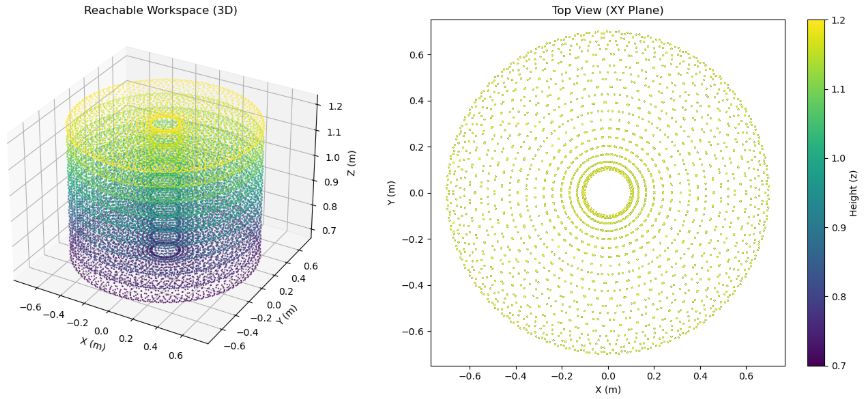
\includegraphics[width=0.8\textwidth]{3D2D.png}
	\caption{نمودارهای فضای کاری ربات در حالت سه‌بعدی و نمای بالا}
\end{figure}


\paragraph{تحلیل و تفسیر نمودار سه‌بعدی فضای کاری}\mbox{}\\
تصویر سمت چپ در خروجی (\lr{Reachable Workspace (3D)})، شکل کلی فضای کاری ربات را به صورت یک استوانه توخالی (لوله‌ای ضخیم) نشان می‌دهد. 
رنگ‌بندی این نقاط بر اساس محور $Z$ (ارتفاع) صورت گرفته است. همان‌طور که نوار رنگ (\lr{Colorbar}) نشان می‌دهد، پایین‌ترین نقاط (رنگ بنفش تیره) مربوط به ارتفاع $0.7$ متر هستند که معادل حالتی است که مفصل کشویی اول بسته است ($q_1 = 0 \Rightarrow z = D_0 = 0.7$). بالاترین نقاط (رنگ زرد) مربوط به ارتفاع $1.2$ متر هستند که معادل باز شدن کامل مفصل کشویی است ($q_1 = 0.5 \Rightarrow z = 0.7 + 0.5 = 1.2$). بنابراین، حرکت مفصل اول ($q_1$) صرفاً این فضای کاری را در امتداد محور $Z$ جابجا می‌کند و استوانه را شکل می‌دهد.

\paragraph{تحلیل دقیق نمای بالا (صفحه \LR{XY}) و مرزهای فضای کاری}\mbox{}\\
تصویر سمت راست (\lr{Top View}) تصویر فضای کاری روی صفحه $XY$ را نشان می‌دهد که دقیقاً شبیه به یک «دونات» (حلقه) است. این شکل حاصل دوران مفاصل لولایی دوم و سوم ($q_2$ و $q_3$) است.
دو مرز بسیار مهم در این نمودار قابل مشاهده و تحلیل ریاضی هستند:
\begin{itemize}
	\item \textbf{مرز خارجی (حداکثر دسترسی):} این مرز زمانی شکل می‌گیرد که بازوهای دوم و سوم کاملاً در یک راستا و کشیده باشند؛ یعنی زاویه مفصل سوم صفر باشد ($q_3 = 0$). در این حالت، شعاع دسترسی ربات برابر با مجموع طول دو بازو است. با توجه به مقادیر داده‌شده، شعاع خارجی برابر است با $R_{max} = L_2 + L_3 = 0.4 + 0.3 = 0.7$ متر. اگر به محورهای مختصات $X$ و $Y$ در تصویر سمت راست دقت کنید، مشخص است که دورترین نقاط دقیقاً روی دایره‌ای به شعاع $0.7$ قرار گرفته‌اند (از $-0.7$ تا $+0.7$).
	\item \textbf{مرز داخلی (حفره وسط فضای کاری):} این بخش، ناحیه‌ای در اطراف پایه ربات است که نوک ابزار هرگز نمی‌تواند به آن برسد. این مرز زمانی شکل می‌گیرد که لینک سوم کاملاً به سمت داخل تا شود؛ یعنی زاویه مفصل سوم $q_3 = 180^\circ$ یا $\pi$ رادیان باشد. در این حالت شعاع دسترسی به کمترین مقدار خود می‌رسد که برابر با قدر مطلق تفاضل طول دو بازو است: $R_{min} = |L_2 - L_3| = |0.4 - 0.3| = 0.1$ متر. این اختلاف دقیقاً شعاع سوراخ وسط دونات را تشکیل می‌دهد. در نمودار سمت راست، به وضوح یک فضای خالی دایره‌ای در مرکز به شعاع $0.1$ متر دیده می‌شود.
\end{itemize}
بنابراین، این نمودارها با دقت بالایی رفتار سینماتیکی ربات را تایید کرده و نشان می‌دهند که ربات در صفحه افقی تنها می‌تواند در یک نوار حلقوی بین شعاع $0.1$ تا $0.7$ متریِ خود عملیات انجام دهد.
\subsubsection{تسک \lr{B.5} — رسیدن به قطعات با روش جستجوی سینماتیک مستقیم}
\paragraph{شرح پیاده‌سازی و روش کار}\mbox{}\\
در این تسک، هدف قرار دادن مجری نهایی ربات در بالای سرِ دیسک‌های شناسایی‌شده در بخش بینایی ماشین است. این کار طی دو مرحله انجام می‌شود. مرحله اول تنظیم ارتفاع ربات است؛ با توجه به اینکه ارتفاع ایمن بالای میز $z_{safe} = 0.05$ متر در نظر گرفته شده و رابطه ارتفاع ربات $z_E = D_0 + q_1$ است، با یک محاسبه ساده جبری می‌توان مقدار مفصل کشویی را به صورت $q_1 = z_{safe} - D_0$ به دست آورد و ارتفاع را تنظیم کرد.
مرحله دوم، یافتن زوایای مناسب برای مفاصل دورانی ($q_2$ و $q_3$) است تا ربات در مختصات صفحه‌ای ($x, y$) مورد نظر قرار گیرد. از آنجایی که در این بخش استفاده از سینماتیک معکوس مجاز نیست، از روش جستجوی جامع شبکه (\lr{Brute-force grid search}) روی معادلات سینماتیک مستقیم استفاده شده است. در این روش، بازه حرکتی هر دو مفصل دورانی (از $-\pi$ تا $\pi$) به ۲۵۰ نقطه تقسیم شده است. الگوریتم تمام ترکیبات ممکن برای زوایا را در معادلات سینماتیک مستقیم قرار داده و خطای اقلیدسی (فاصله) بین مختصات حاصل و مرکز هدف را محاسبه می‌کند. در نهایت، زوج زاویه‌ای که کمترین خطا را تولید کند به عنوان جواب برگردانده می‌شود.

\paragraph{کد پایتون پیاده‌سازی‌شده}\mbox{}\\
کد زیر پیاده‌سازی روش جستجوی جامع شبکه برای یافتن زوایای مناسب مفاصل و بررسی میزان خطای نهایی را نشان می‌دهد:
\addcontentsline{lol}{lstlisting}{کد تسک \lr{B.5}}
\begin{latin}
\begin{LTR}
\begin{minted}{python}
	import numpy as np
	
	# Robot physical parameters
	D0, L2, L3 = 0.70, 0.40, 0.30
	
	# Data of detected disks from computer vision (Section A)
	my_data = [
	{'color': 'red', 'xy': (0.186, -0.104)},
	{'color': 'red', 'xy': (0.103, 0.052)},
	{'color': 'green', 'xy': (-0.053, 0.208)},
	{'color': 'green', 'xy': (-0.156, 0.072)},
	{'color': 'blue', 'xy': (-0.229, -0.186)}
	]
	
	def find_best_ik(tx, ty, L2, L3):
	"""Finds optimal q2 and q3 using a grid search (Brute-force)."""
	best_err = float('inf')
	best_q = (0, 0)
	
	# Sampling range for joint angles
	q2_samples = np.linspace(-np.pi, np.pi, 250)
	q3_samples = np.linspace(-np.pi, np.pi, 250)
	
	for q2 in q2_samples:
	for q3 in q3_samples:
	# Forward kinematics for the planar 2R part
	x = L2 * np.cos(q2) + L3 * np.cos(q2 + q3)
	y = L2 * np.sin(q2) + L3 * np.sin(q2 + q3)
	
	# Euclidean distance error
	dist = np.sqrt((x - tx)**2 + (y - ty)**2)
	
	if dist < best_err:
	best_err = dist
	best_q = (q2, q3)
	
	return best_q, best_err
	
	# Execution and Result Formatting
	print(f"{'Color':<8} | {'Coordinates (m)':<18} | {'Error (m)':<10} | {'Status'}")
	print("-" * 55)
	
	for disk in my_data:
	tx, ty = disk['xy']
	
	# Perform IK search
	q_sol, err = find_best_ik(tx, ty, L2, L3)
	
	# Check if error is within the 5mm threshold
	reachable = err < 0.005
	status = "Success" if reachable else "Out of Range"
	
	print(f"{disk['color']:<8} | ({tx:>6.3f}, {ty:>6.3f}) | {err:.5f}   | {status}")
\end{minted}
\end{LTR}
\end{latin}

\paragraph{نتایج و تحلیل بررسی خطاها}\mbox{}\\
با اجرای کد فوق، خروجی زیر برای ۵ دیسک هدف حاصل شد:

\begin{latin}
	\begin{verbatim}
	Color    | Coordinates (m)    | Error (m)  | Status
-------------------------------------------------------
	red      | ( 0.186, -0.104) | 0.00163   | Success
	red      | ( 0.103,  0.052) | 0.00226   | Success
	green    | (-0.053,  0.208) | 0.00106   | Success
	green    | (-0.156,  0.072) | 0.00067   | Success
	blue     | (-0.229, -0.186) | 0.00352   | Success
	\end{verbatim}
\end{latin}

با بررسی جدول خروجی، به وضوح مشاهده می‌شود که ستون خطای موقعیت (\lr{Error}) برای تمام دیسک‌ها مقداری در محدوده $0.00067$ تا $0.00352$ متر (معادل $0.67$ تا $3.52$ میلی‌متر) دارد. از آنجایی که حد آستانه مجاز برای خطا در صورت سوال برابر با ۵ میلی‌متر ($0.005$ متر) تعیین شده بود، تمامی خطاهای به‌دست‌آمده کاملاً زیر این حد مجاز قرار دارند.
بیشترین خطا مربوط به دیسک آبی‌رنگ با مقدار $3.52$ میلی‌متر است که همچنان به شکل قابل‌توجهی کمتر از ۵ میلی‌متر است. این نتایج تایید می‌کنند که الگوریتم جستجوی جامعِ شبکه‌ای، با رزولوشن انتخاب‌شده برای نمونه‌برداری (۲۵۰ نمونه در هر زاویه)، عملکرد بسیار خوبی داشته و توانسته است ربات را با خطای بسیار ناچیز و قابل‌قبولی به دقت در بالای سرِ تمامی دیسک‌ها قرار دهد (وضعیت \lr{Success} برای همه اهداف).

\subsection{بخش \lr{D} --- سوالات تحلیلی}
\subsubsection{پاسخ سوال اول}

از آنجا که مفصل اول ربات \lr{PRR} از نوع کشویی است و تنها ارتفاع ربات را در راستای محور $ z $ تغییر می دهد، شعاع دسترسی ربات روی سطح میز توسط دو مفصل دورانی بعدی ($ q_2 $ و $ q_3 $) و طول لینک های آن ها ($ L_2 $ و $ L_3 $) تعیین می شود. مفهوم کلیدی در اینجا نامساوی مثلث (\lr{Triangle Inequality}) در هندسه اقلیدسی است که مرزهای داخلی و خارجی این فضای کاری را شکل می دهد.

تصویر حرکت مفاصل دوم و سوم ربات روی صفحه افقی $ xy $، معادل یک مکانیزم بازوی صفحه ای دو لینکی (\lr{Planar Two-Link Manipulator}) است. اگر مبدا مختصات (پایه ربات) را نقطه اول، مفصل سوم (آرنج) را نقطه دوم، و افکتور نهایی (نوک ابزار) را نقطه سوم در نظر بگیریم، این سه نقطه رئوس یک مثلث را در صفحه افقی تشکیل می دهند. طول دو ضلع این مثلث ثابت و برابر با $ L_2 $ و $ L_3 $ است.

بر اساس قضیه نامساوی مثلث در هندسه، طول ضلع سوم (یعنی فاصله مستقیم افکتور نهایی از مبدا مختصات که آن را با $ r $ نشان می دهیم) بین قدر مطلق تفاضل و مجموع طول دو ضلع دیگر قرار دارد:

\[
|L_2 - L_3| \le r \le L_2 + L_3
\]

این رابطه ریاضی نشان می دهد که فضای کاری ربات روی یک صفحه دوبعدی، یک دایره توپر نیست، بلکه یک ناحیه حلقوی یا دونات شکل است. 

مرز خارجی حلقه ($ L_2 + L_3 $): زمانی به دست می آید که بازوی ربات کاملا باز و کشیده باشد. در این حالت، زاویه مفصل سوم $ q_3 = 0 $ بوده و دو لینک در یک امتداد قرار می گیرند. در نتیجه ابزار ربات به بیشترین فاصله از پایه می رسد.

مرز داخلی حلقه ($ |L_2 - L_3| $): زمانی به دست می آید که مفصل سوم کاملا به سمت داخل تا شود ($ q_3 = \pi $ یا $ q_3 = -\pi $). در این حالت، لینک سوم روی لینک دوم برمی گردد و افکتور نهایی در نزدیک ترین فاصله نسبت به پایه قرار می گیرد. 

\paragraph{ارتباط با ابعاد میز و ناحیه پوشش داده شده}\mbox{}\\
دلیل اینکه ابعاد میز تحت پوشش ربات با عبارت $ |L_2 - L_3| $ مقیاس دهی شده و به آن بستگی دارد، وجود یک ناحیه کور در مرکز میز کار است. 

محدوده به شعاع $ |L_2 - L_3| $ در مرکز مختصات، یک استوانه غیرقابل دسترس را تشکیل می دهد. اگر ربات در مرکز یک میز کار نصب شده باشد، نمی تواند قطعاتی که در دایره ای به شعاع $ |L_2 - L_3| $ از مرکز قرار دارند را بازرسی کند. 

بنابراین، اگر قرار باشد ربات تمام سطح یک میز مشخص را پوشش دهد، آن میز نباید شامل نقطه ای در داخل دایره $ |L_2 - L_3| $ باشد و در عین حال نباید از مرز $ L_2 + L_3 $ فراتر برود. اگر می خواستیم ربات نقطه کوری در مرکز نداشته باشد، از نظر هندسی باید طول دو لینک برابر در نظر گرفته می شد (یعنی $ L_2 = L_3 $ که نتیجه آن $ |L_2 - L_3| = 0 $ است). از آنجا که در این مسئله $ L_2 $ و $ L_3 $ متفاوت هستند، هندسه و شعاع داخلی منطقه ای که ربات توانایی پوشش آن را دارد، به عبارت تفاضل این دو طول مقیاس شده و مرتبط است.
\subsubsection{پاسخ سوال دوم}
برای کاهش هزینه‌ی جستجو در الگوریتم با پیچیدگی زمانی $\mathcal{O}(N^2)$ می‌توان از روش \lr{Precomputed Lookup Table} استفاده کرد.

ایده‌ی اصلی این است که به‌جای حل معادلات سینماتیک معکوس برای هر هدف به‌صورت جداگانه یک بار پیش‌پردازش روی فضای پیکربندی \lr{(configuration space)} ربات انجام دهیم.

\paragraph{جدول جستجوی پیش‌محاسبه‌شده}\mbox{}\\
برای بازوی \lr{PRR}، فضای پیکربندی شامل سه متغیر مفصلی است:
$$\mathbf{q} = (d_1,\, \theta_2,\, \theta_3)$$
که $d_1$ جابه‌جایی کشویی و $\theta_2, \theta_3$ زوایای مفاصل دورانی هستند.

در مرحله‌ی اول از پیش‌پردازش، فضای پیکربندی را با گام‌های گسسته نمونه‌برداری می‌کنیم. سپس به ازای هر پیکربندی $\mathbf{q}_i$، سینماتیک مستقیم \lr{(forward kinematics)} را محاسبه و موقعیت نوک ابزار $\mathbf{p}_i = f(\mathbf{q}_i)$ را به دست می‌آوریم:
\[
    \mathbf{p}_i = f(\mathbf{q}_i) \in \mathbb{R}^2, \quad i = 1, 2, \ldots, N
\]

در مرحله‌ی دوم، جدولی به شکل $\{(\mathbf{p}_i,\, \mathbf{q}_i)\}$ می‌سازیم و آن را در یک ساختار \lr{k-d tree} یا \lr{hash grid} ذخیره می‌کنیم تا جستجوی نزدیک‌ترین همسایه \lr{(nearest neighbor search)} با پیچیدگی $\mathcal{O}(\log N)$ ممکن شود.

در مرحله‌ی سوم، برای هر هدف جدید $\mathbf{p}^*$ (از جمله ۳۰ قطعه روی میز)، نزدیک‌ترین نقطه‌ی از پیش محاسبه‌شده را از جدول استخراج می‌کنیم:
\[
    \mathbf{q}^* = \arg\min_{\mathbf{q}_i} \|\mathbf{p}_i - \mathbf{p}^*\|_2
\]

\paragraph{تحلیل هزینه}\mbox{}\\
هزینه‌ی پیش‌پردازش یک‌بار انجام می‌شود و برابر است با:
\[
    T_{\text{pre}} = \mathcal{O}(N^2)
\]

پس از آن، هزینه‌ی جستجو برای هر یک از $M = 30$ هدف برابر است با:
\[
    T_{\text{query}} = \mathcal{O}(M \log N)
\]

بنابراین هزینه‌ی کل \lr{amortize} شده برای همه‌ی اهداف برابر است با:
\[
    T_{\text{total}} = \mathcal{O}(N^2 + M \log N)
\]

که در آن جمله‌ی $\mathcal{O}(N^2)$ تنها یک‌بار پرداخت می‌شود و هزینه‌ی آن بین تمام $M$ هدف سرشکن \lr{(amortise)} می‌گردد.
میانگین هزینه‌ی هر هدف به‌صورت زیر کاهش می‌یابد:
\[
    \bar{T} = \mathcal{O}\!\left(\frac{N^2}{M} + \log N\right)
\]

برای $M = 30$، این کاهش کاملاً محسوس است.
\subsubsection{پاسخ سوال سوم}

\paragraph{۱. اعوجاج شعاعی \lr{(Radial Distortion)}}\mbox{}\\

شایع‌ترین نوع اعوجاج لنز است. در این نوع اعوجاج که شایع‌ترین نوع اعوجاج لنز است، نقاط تصویر در راستای شعاعی نسبت به مرکز اپتیکال جابه‌جا می‌شوند. مدل ریاضی آن به صورت زیر است:
\[
    x' = x(1 + k_1 r^2 + k_2 r^4 + k_3 r^6)
\]
\[
    y' = y(1 + k_1 r^2 + k_2 r^4 + k_3 r^6)
\]
که در آن $r^2 = x^2 + y^2$ فاصله‌ی شعاعی از مرکز تصویر و $k_1, k_2, k_3$ ضرایب اعوجاج شعاعی هستند. اگر $k_1 < 0$ باشد، اعوجاج بشکه‌ای \lr{(barrel distortion)} و اگر $k_1 > 0$ باشد، اعوجاج بالشتکی \lr{(pincushion distortion)} رخ می‌دهد.
\paragraph{۲. اعوجاج مماسی \lr{(Tangential Distortion)}}\mbox{}\\
ناشی از عدم موازی بودن کامل صفحه‌ی لنز با صفحه‌ی سنسور است:
\[
    x' = x + \left[2p_1 xy + p_2(r^2 + 2x^2)\right]
\]
\[
    y' = y + \left[p_1(r^2 + 2y^2) + 2p_2 xy\right]
\]
که $p_1, p_2$ ضرایب اعوجاج مماسی هستند.

\paragraph{۳. سایر اعوجاج‌های محیط صنعتی}\mbox{}\\
علاوه بر موارد فوق، در محیط‌های صنعتی با موارد زیر نیز مواجه هستیم:
\begin{itemize}
\item انحراف کروی \lr{(Spherical Aberration)}: شعاع‌های نوری حاشیه‌ی لنز در نقطه‌ی کانونی متفاوتی نسبت به شعاع‌های مرکزی تمرکز می‌یابند.
\item 
انحراف رنگی \lr{(Chromatic Aberration)}: طول موج‌های مختلف نور در نقاط کانونی متفاوت متمرکز می‌شوند که منجر به حاشیه‌های رنگی در لبه‌های اجسام می‌گردد.
\end{itemize}



تصحیح اعوجاج لنز باید اولین مرحله‌ی پایپ‌لاین، پیش از هر پردازش دیگری، قرار گیرد. دلیل این امر آن است که اعوجاج لنز یک خطای سیستماتیک در سطح سنسور است و تمام مراحل بعدی از جمله تصحیح پرسپکتیو، آشکارسازی نشانگرها \lr{(markers)} و تخمین وضعیت \lr{(pose estimation)} بر فرض هندسه‌ی تصویر ایده‌آل بنا شده‌اند.

\subsubsection{سوال چهارم}
خطای آفست سیستماتیک (\lr{Systematic Offset}) به معنای یک انحراف ثابت، قابل پیش‌بینی و تکرارپذیر بین خروجی مدل ریاضی (سینماتیک مستقیم تحلیلی) و خروجی شبیه‌ساز است. اگر در ساخت فایل \lr{URDF} اشتباهاتی رخ دهد که ساختار هندسی یا دستگاه‌های مختصات را نسبت به قراردادهای ریاضی (مانند پارامترهای \lr{DH}) جابه‌جا کند، این نوع خطا در خروجی تابع \lr{getLinkState} ایجاد می‌شود. مهم‌ترین دلایل هندسی و ساختاری بروز این خطا عبارتند از:

۱. عدم تطابق در بردار انتقال و دوران مفاصل (\lr{Joint Origin Misalignment}):
در ساختار \lr{URDF}، موقعیت هر لینک نسبت به لینک قبلی توسط تگ \lr{<origin xyz="..." rpy="...">} در داخل تعریفِ مفصل (\lr{<joint>}) مشخص می‌شود. این مقادیر مستقیما بیانگر طول لینک‌ها و زوایای انحراف مفصلی در معادلات \lr{DH} هستند. اگر مقدار وارد شده در فایل \lr{URDF} (مثلا طول لینک دوم $ L_2 $) حتی چند میلی‌متر با مقادیر ثابت دستگاه معادلات تحلیلی تفاوت داشته باشد، یک خطای انتقال ثابت به تمامی لینک‌های بعدی زنجیره سینماتیکی اعمال شده و خطای آفست ایجاد می‌کند.

۲. تداخل فریم مرکز جرم با فریم سینماتیکی (\lr{CoM vs. URDF Link Frame}):
تابع \lr{getLinkState} در کتابخانه \lr{PyBullet} تاپلی از چندین خروجی را باز می‌گرداند. ایندکس $ 0 $ مختصات مرکز جرم (\lr{Center of Mass Position}) را در فضای جهانی نشان می‌دهد، در حالی که ایندکس $ 4 $ مختصات دقیق مبدا دستگاه متصل به لینک (\lr{World Link Frame Position}) را بازمی‌گرداند. اگر در فایل \lr{URDF}، درون تگ \lr{<inertial>} مقدار \lr{<origin>} غیر صفر تعریف شده باشد و شما به اشتباه ایندکس $ 0 $ را با معادلات ریاضی خود مقایسه کنید، دقیقا به اندازه بردار انتقالِ مرکز جرم، یک خطای سیستماتیک در تمام خروجی‌ها مشاهده خواهید کرد.

۳. اشتباه در تعریف مفصل مجازیِ افکتور نهایی (\lr{End-effector Dummy Link}):
نقطه ابزار یا افکتور نهایی در سینماتیک معمولاً به عنوان یک نقطه ریاضی در انتهای لینک آخر در نظر گرفته می‌شود. برای استخراج این نقطه در \lr{URDF}، عموماً یک مفصل ثابت (\lr{Fixed Joint}) بدون جرم و یک لینک مجازی تعریف می‌شود. اگر فاصله و جهت این مفصل ثابت با آنچه در ماتریس انتقال نهایی (برای مثال ماتریس $ T_3^0 $) فرض شده است، همخوانی نداشته باشد (مثلا آفست نوک ابزار صفر فرض شده باشد اما در \lr{URDF} مقداری به آن اختصاص یابد)، خطای آفست سیستماتیک در فضای دکارتی پدیدار می‌شود.

۴. جابه‌جایی مبدا لینک پایه (\lr{Base Frame Offset}):
اگر فایل \lr{URDF} به گونه‌ای طراحی شده باشد که مبدا مختصات لینک پایه ربات با مبدا هندسی مفصل اول (یا سطح میز کار) دقیقا منطبق نباشد، یا هنگام فراخوانی تابع بارگذاری ربات در محیط \lr{PyBullet}، ربات دقیقا در مختصات $ (0, 0, 0) $ و بدون دوران اولیه قرار نگیرد، تمام محاسبات استخراج شده توسط \lr{getLinkState} دارای یک شیفت سراسری و سیستماتیک نسبت به مختصات جهانیِ محاسبات تحلیلی خواهند بود.

\subsubsection{سوال پنجم}
در پیکربندی \lr{Eye-in-Hand}، دوربین به جای یک نقطه ثابت در محیط، به صورت صلب روی یکی از لینک‌های متحرک ربات (در این مسئله، مفصل دوم) نصب می‌شود. در نتیجه، موقعیت و زاویه دید دوربین در هر لحظه به وضعیت مفاصل پیش از خود (یعنی مفصل کشویی $ q_1 $ و مفصل دورانی $ q_2 $) بستگی دارد. برای استخراج موقعیت قطعات روی میز کار صرفاً با استفاده از سینماتیک مستقیم، پایپ‌لاین به شرح زیر تغییر می‌کند:

۱. محاسبه موقعیت و جهت‌گیری دوربین در فضای جهانی:
ابتدا مقادیر فعلی مفاصل $ q_1 $ و $ q_2 $ خوانده می‌شود. با قرار دادن این مقادیر در معادلات سینماتیک مستقیم (\lr{Forward Kinematics})، ماتریس تبدیلِ همگنِ مفصل دوم نسبت به دستگاه پایه ربات به دست می‌آید. از آنجا که دوربین به صورت صلب به این مفصل متصل است، یک ماتریس تبدیل ثابت هندسی (آفست نصب دوربین) نیز وجود دارد. حاصل‌ضرب ماتریس سینماتیک مستقیم در این ماتریس ثابت، موقعیت و زاویه دقیق لنز دوربین را در دستگاه مختصات پایه ربات مشخص می‌کند.

۲. پردازش تصویر و تشکیل پرتوهای نوری:
تصویر گرفته شده توسط دوربین با استفاده از الگوریتم‌های بینایی ماشین (مشابه بخش‌های قبل) پردازش می‌شود تا مختصات پیکسلی $ (u, v) $ برای مرکز هر دیسک رنگی پیدا شود. با استفاده از پارامترهای ذاتی دوربین (\lr{Intrinsic Parameters})، این مختصات دوبعدیِ پیکسلی به یک پرتو برداریِ سه‌بعدی (\lr{Ray}) در دستگاه مختصات محلیِ دوربین (\lr{Camera Frame}) نگاشت می‌شود.

۳. انتقال پرتوها به دستگاه پایه ربات:
با استفاده از موقعیت دوربین که در مرحله اول از طریق سینماتیک مستقیم به دست آمد، امتداد این پرتوهای نوری از دستگاه محلیِ دوربین به دستگاه مختصاتِ جهانی یا پایه ربات (\lr{Base Frame}) منتقل می‌شود. اکنون ما یک خط سه‌بعدی در فضای واقعی داریم که از لنز دوربین شروع شده و از مرکز هدف عبور می‌کند.

۴. تقاطع هندسی با صفحه کار (یافتن مختصات نهایی):
از اطلاعات مسئله می‌دانیم که تمام قطعات روی سطح صاف میز کار قرار دارند و سطح میز دقیقاً معادل صفحه $ z = 0 $ در دستگاه مختصات جهانی است. برای یافتن موقعیت دقیق قطعه، صرفاً کافی است محل برخوردِ پرتوِ سه‌بعدیِ منتقل شده به فضای جهانی را با صفحه $ z = 0 $ محاسبه کنیم. نقطه تقاطع، دقیقاً مختصات $ x $ و $ y $ قطعات را روی میز به دست می‌دهد. 

به این ترتیب، کل فرآیند تبدیل پیکسل به مختصات ربات، بدون نیاز به حل سینماتیک معکوس و تنها با یک استفاده مستقیم از معادلات سینماتیک مستقیم و یک تقاطع خط و صفحه، پیاده‌سازی می‌گردد.

\end{document}

